\documentclass{beamer}
\usepackage{natbib}
\usepackage{wrapfig}

%Set unseen sections to no shading (as TOC is only used as TOC)
\setbeamertemplate{section in toc shaded}[default][100]
\setbeamertemplate{subsection in toc shaded}[default][100]

%Fix the appendix: style it like a table of contents
%Find reference: Alexandersson, H., and A. Moberg, 1997: Homogenization of Swedish temperature data. Part I: Homogeneity test for linear trends. Int. J. Climatol., 17, 25–34. \cite{alexandersson97}

\def\bbeta{{\boldsymbol \beta}}
\def\bepsilon{{\boldsymbol \epsilon}}

\begin{document}

\title{Simultaneous Treatment of Random and Systematic Errors in the Historical Radiosonde Temperature Archive}
\author{Josh Browning}
\date{\today}

\frame{\titlepage} 

\part{1}

\frame{\frametitle{Table of contents}\tableofcontents[currentsection]} 

\section{Problem}

\frame{
\frametitle{Project Overview}
\textbf{Problem:} Random and systematic errors exist in the radiosonde temperature archive, and no studies have addressed how to handle both types of errors simultaneously.\\
\textbf{Solution:}  I studied the effect of applying various sequences of quality control algorithms on simulated data which was designed to have the same structure as true radiosonde data.
}	

\subsection{Random Errors}

\frame{\frametitle{Problems with the radiosonde data: Random Errors}
	\begin{columns}
		\begin{column}{.4\textwidth}
			Random errors can occur because of
			\begin{enumerate}
				\item Faulty data transmission
				\item Sporadic instrumentation problems
				\item Keystroke entries
				\item Errors in data management
				\item Many other reasons
			\end{enumerate}
		\end{column}
		\begin{column}{.6\textwidth}
			\begin{figure}
				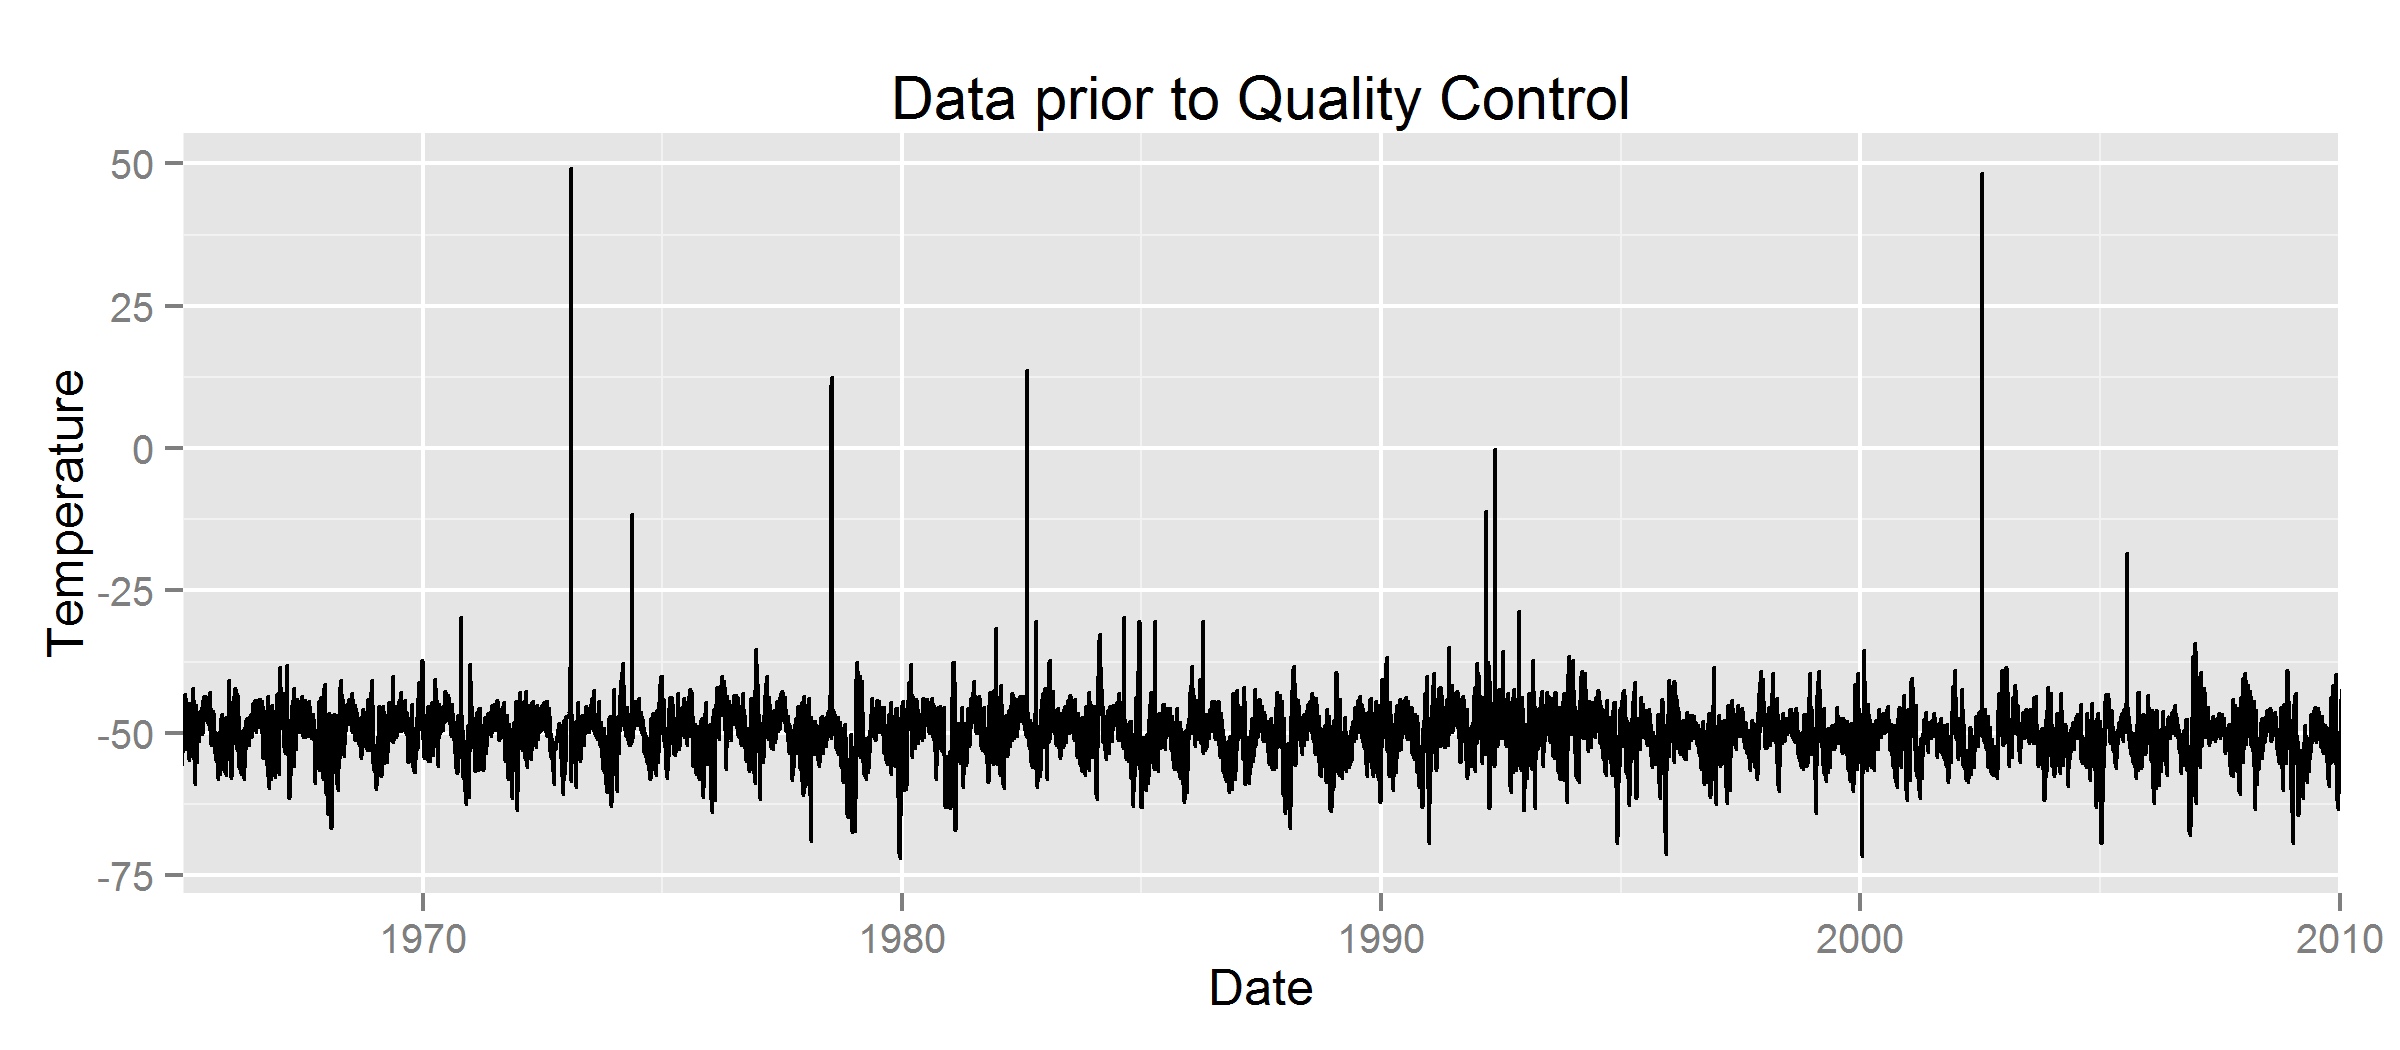
\includegraphics[width=\textwidth]{70219_Data_Unhomogenized_no_vlines}
				\label{fig:70219_out}
				\caption{Data collected from Station 70219 in Bethel, Alaska.}
			\end{figure}
		\end{column}
	\end{columns}
}

\subsection{Systematic Errors}
\frame{\frametitle{Problems with the radiosonde data: Systematic Errors}
	\begin{columns}
		\begin{column}{.4\textwidth}
			Systematic errors can occur because of
			\begin{enumerate}
				\item Station location changes
				\item Urbanization of the area surrounding the station
				\item Changes in instrumentation
				\item Many other reasons
			\end{enumerate}
		\end{column}
		\begin{column}{.6\textwidth}
			\begin{figure}
				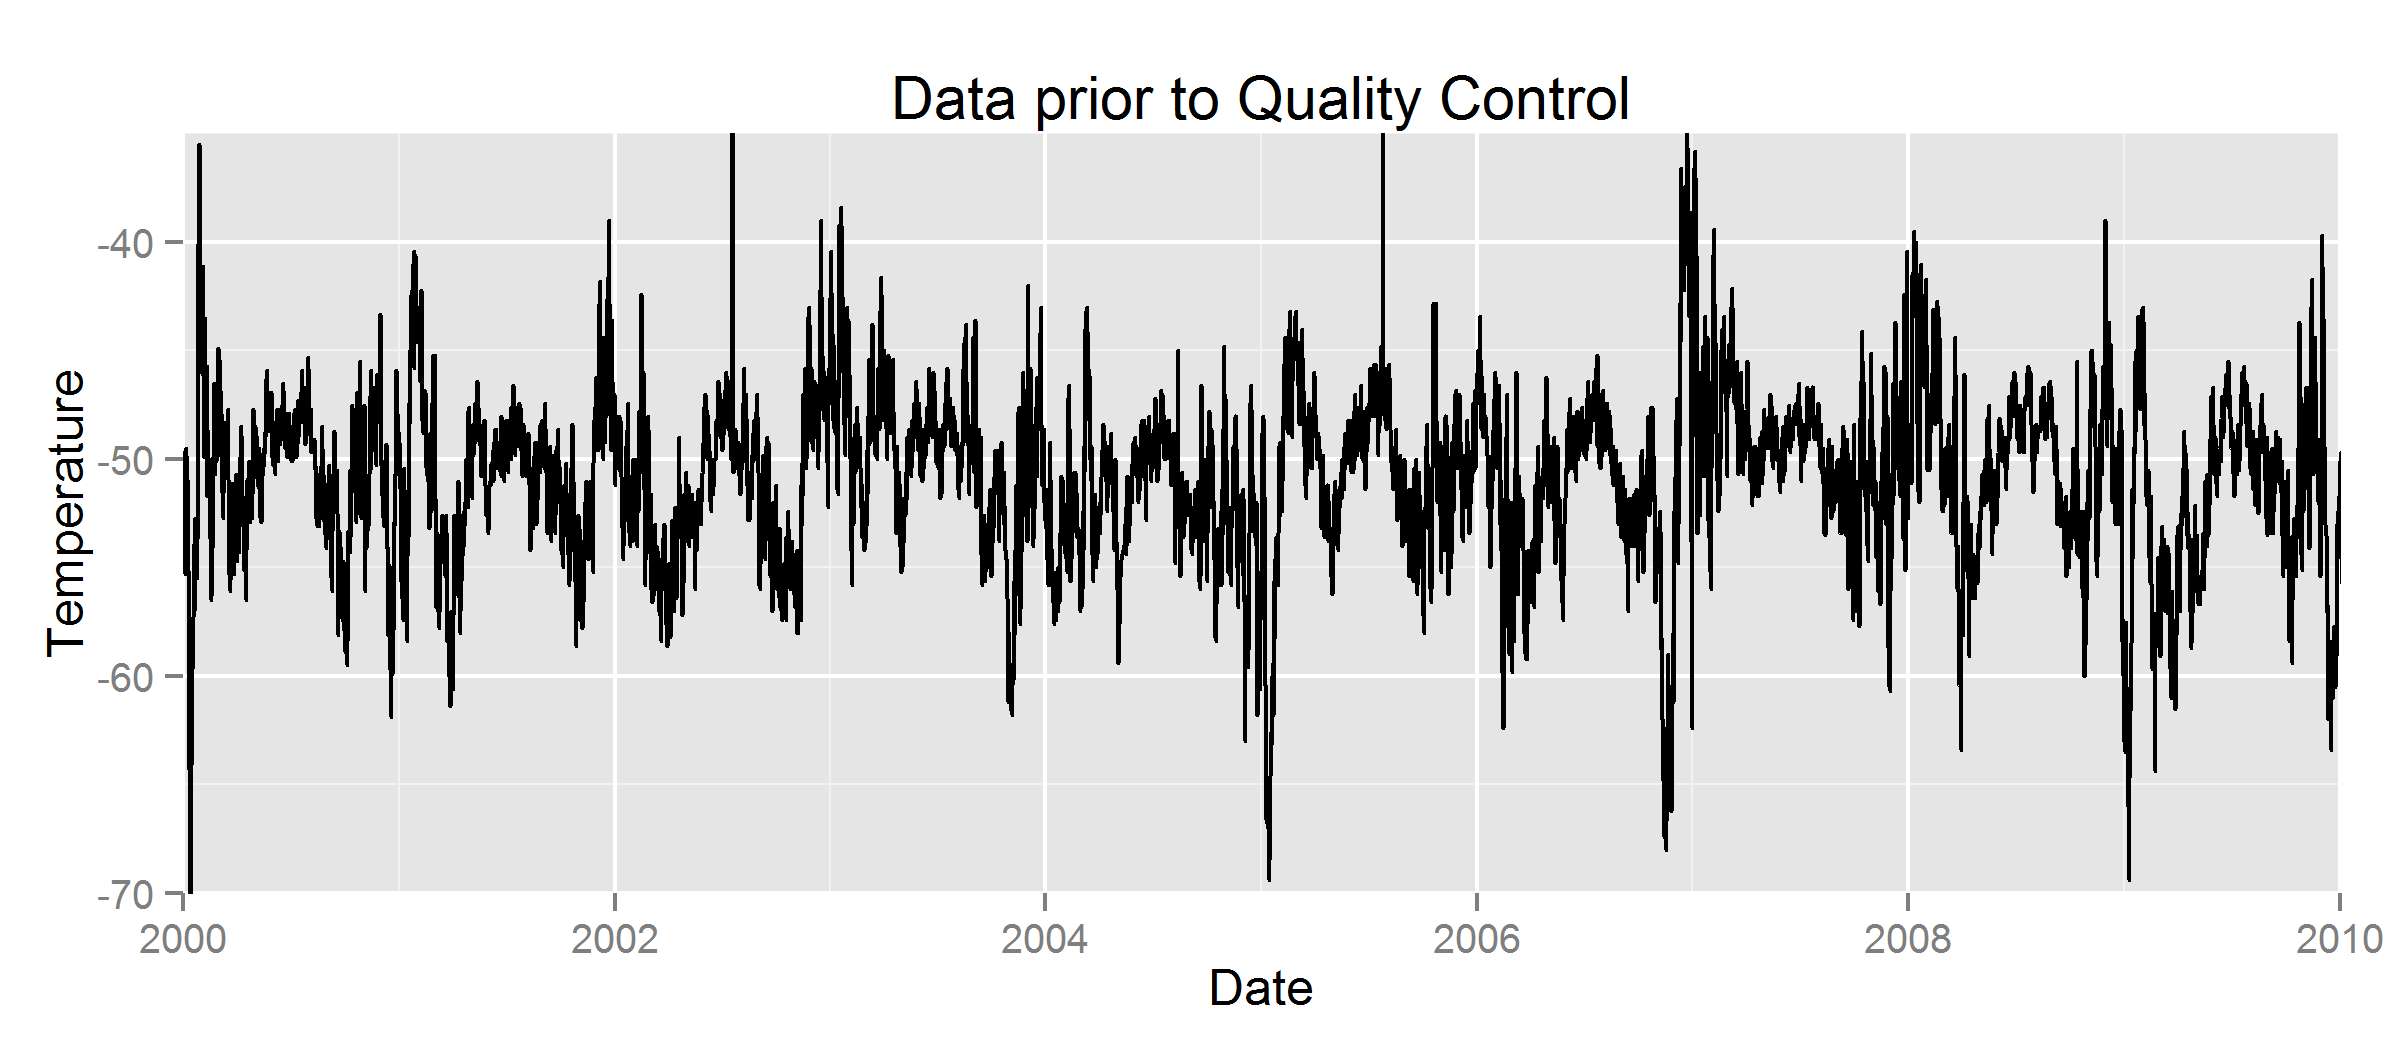
\includegraphics[width=\textwidth]{70219_Data_Unhomogenized_zoomed_no_vlines}
				\label{fig:70219_in}
				\caption{Data collected from Station 70219 in Bethel, Alaska.}
			\end{figure}
		\end{column}
	\end{columns}
}

\frame{\frametitle{Note on terminology}
\begin{tabular}{|p{2cm}|p{4cm}|p{4cm}|}
	\hline
	& \textbf{Statistics} & \textbf{Climatology}\\
	\hline
	\textbf{Random Error} & Any error which causes a measurement to differ from the true value.  It does not necessarily lead to an extreme observation.  & An observation which is incorrect and inconsistent with the rest of the data (in statistical terms, an outlier).\\
	\hline
	\textbf{Systematic Error} & The error for a set of observations whose mean value is biased from the true mean.  The bias does not have to be constant but could follow some trend. & The error for a set of observations whose mean value has shifted from the true mean (i.e. a constant bias has been introduced).  In statistical language, this is a ``change point.''\\
	\hline
\end{tabular}
For the rest of this presentation, I will use the climatological language.
}

\section{Methods}

\subsection{Random Error Detection}
\frame{\frametitle{Random Error Detection Methods}
	\begin{itemize}
		\item The simplest way to detect random errors is to estimate the mean and standard deviation of the data and then to label observations as random errors if they are more than $k$ standard deviations from the mean (where $k$ may be 5 or so).
		\item In \cite{bell14}, a better alternative is proposed which uses robust estimates of the mean and standard deviation.
		\item These estimators, called the winsorized mean and standard devation(s), reduce the influence of extreme observations.
	\end{itemize}
}

\subsection{Systematic Error Correction (Homogenization)}
\frame{\frametitle{Systematic Error Correction (Homogenization)}
	\begin{itemize}
		\item Many homogenization methods have been proposed in the climate literature: \cite{eskridge95, haimberger07, lanzante96, lanzante03, venema12}.  However, these methods are not generally robust to outliers.
		\item Modern homogenization methods are also presented in the statistical literature \cite{killick12, scott74}.
		\item I'll compare the following methods:
		\begin{itemize}
			\item Standard Normal Homogeneity Test (SNHT)
			\item A proposed ``Robust SNHT'', or the SNHT with robust estimators
			\item Binary Segmentation (BinSeg)
			\item Pruned Exact Linear Time (PELT)
		\end{itemize}
	\end{itemize}
}

\frame{\frametitle{Homogenization Methods: SNHT and Robust SNHT}
\begin{figure}
	\includegraphics[width=.8\textwidth]{SNHT_example}
\end{figure}
\vspace{-.5cm}
\begin{itemize}
	\item The SNHT statistic detects systematic errors by comparing the left and right mean to a threshold.
	\item The robust SNHT replaces the mean and standard deviation estimators with robust estimators.
\end{itemize}
}

\frame{\frametitle{Homogenization Methods: BinSeg and PELT}
	\small
	\begin{figure}
		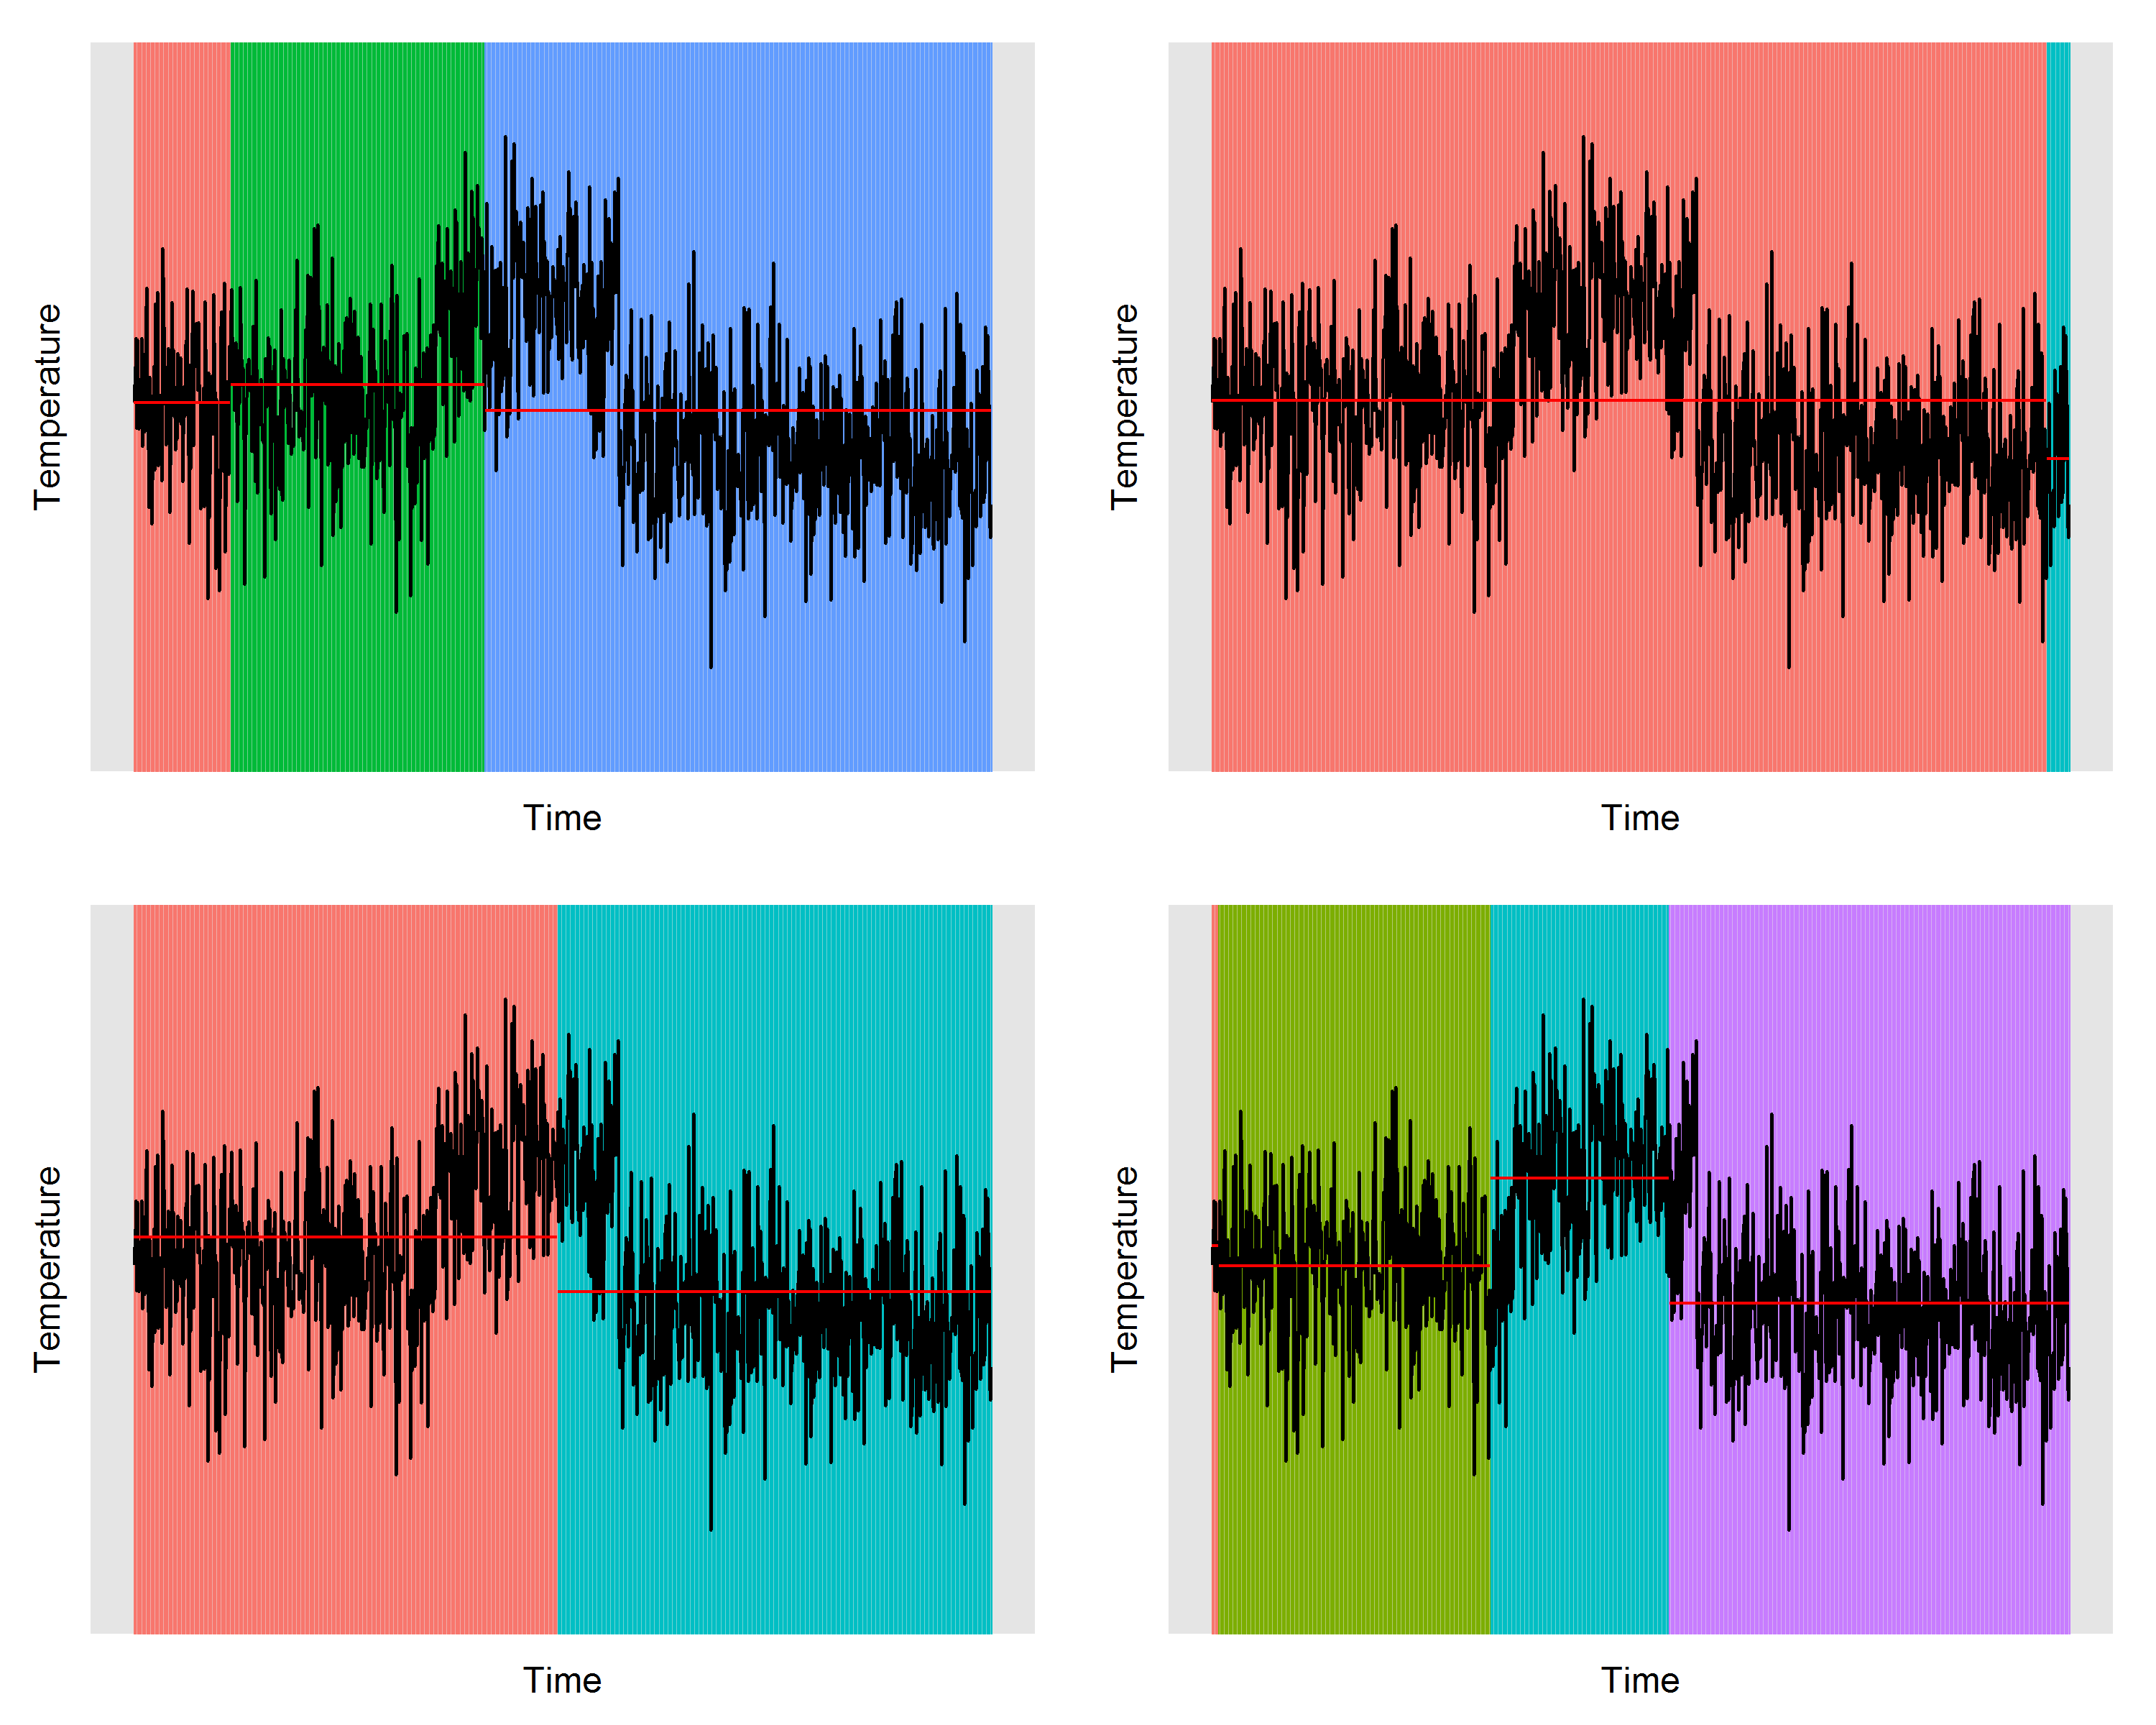
\includegraphics[width=.75\textwidth]{PELT_BinSeg_Example}
	\end{figure}
	\vspace{-.5cm}
	\begin{itemize}
		\item Systematic errors can be detected by optimizing some cost function over all change point configurations.
		\item BinSeg optimizes this function greedily while PELT follows a more sophisticated approach.
	\end{itemize}
}

\subsection{Sequencing}
\frame{\frametitle{Quality Control Algorithm Sequencing}
	\begin{itemize}
		\item I am also interested in understanding the effect that the sequence of the quality control algorithms has on the overall quality control procedure.
		\item Let ``Ran'' denote the random error detection algorithm and ``Sys'' the systematic error correction algorithm.  Then, I investigate the following alternatives:
		\begin{itemize}
			\item Ran$\to$Sys
			\item Sys$\to$Ran
			\item Ran$\to$Sys$\to$Ran
			\item Sys$\to$Ran$\to$Sys
		\end{itemize}
	\end{itemize}
}

\section{Simulation Study}

\subsection{Simulation Design}

\frame{\frametitle{Overall Simulation Design}
	To understand the effect of these various algorithms/sequencings on the final quality controlled dataset, I used the following simulation design:
	\begin{enumerate}
		\item Model observed radiosonde data:
		\begin{itemize}
			\item Fit a GAM to capture daily/seasonal/annual trends
			\item Fit a skew-$t$ distribution to the error terms
			\item Model correlation in the error terms with an AR(1) model.
		\end{itemize}
		\item Simulate a dataset using the model from step 1, and contaminate it with systematic and random errors.
		\item Apply the quality control algorithms described above to the simulated dataset, and determine
		\begin{itemize}
			\item The best homogenization algorithms for sub-daily data in the presence of random errors
			\item The best sequencing in the presence of both random and systematic errors
		\end{itemize}
		\item Repeat steps 2 and 3 1,000 times for each of 10 different radiosonde stations and 3 pressure levels.
	\end{enumerate}
}

\frame{\frametitle{Modeling Radiosonde Data}
	\begin{figure}
		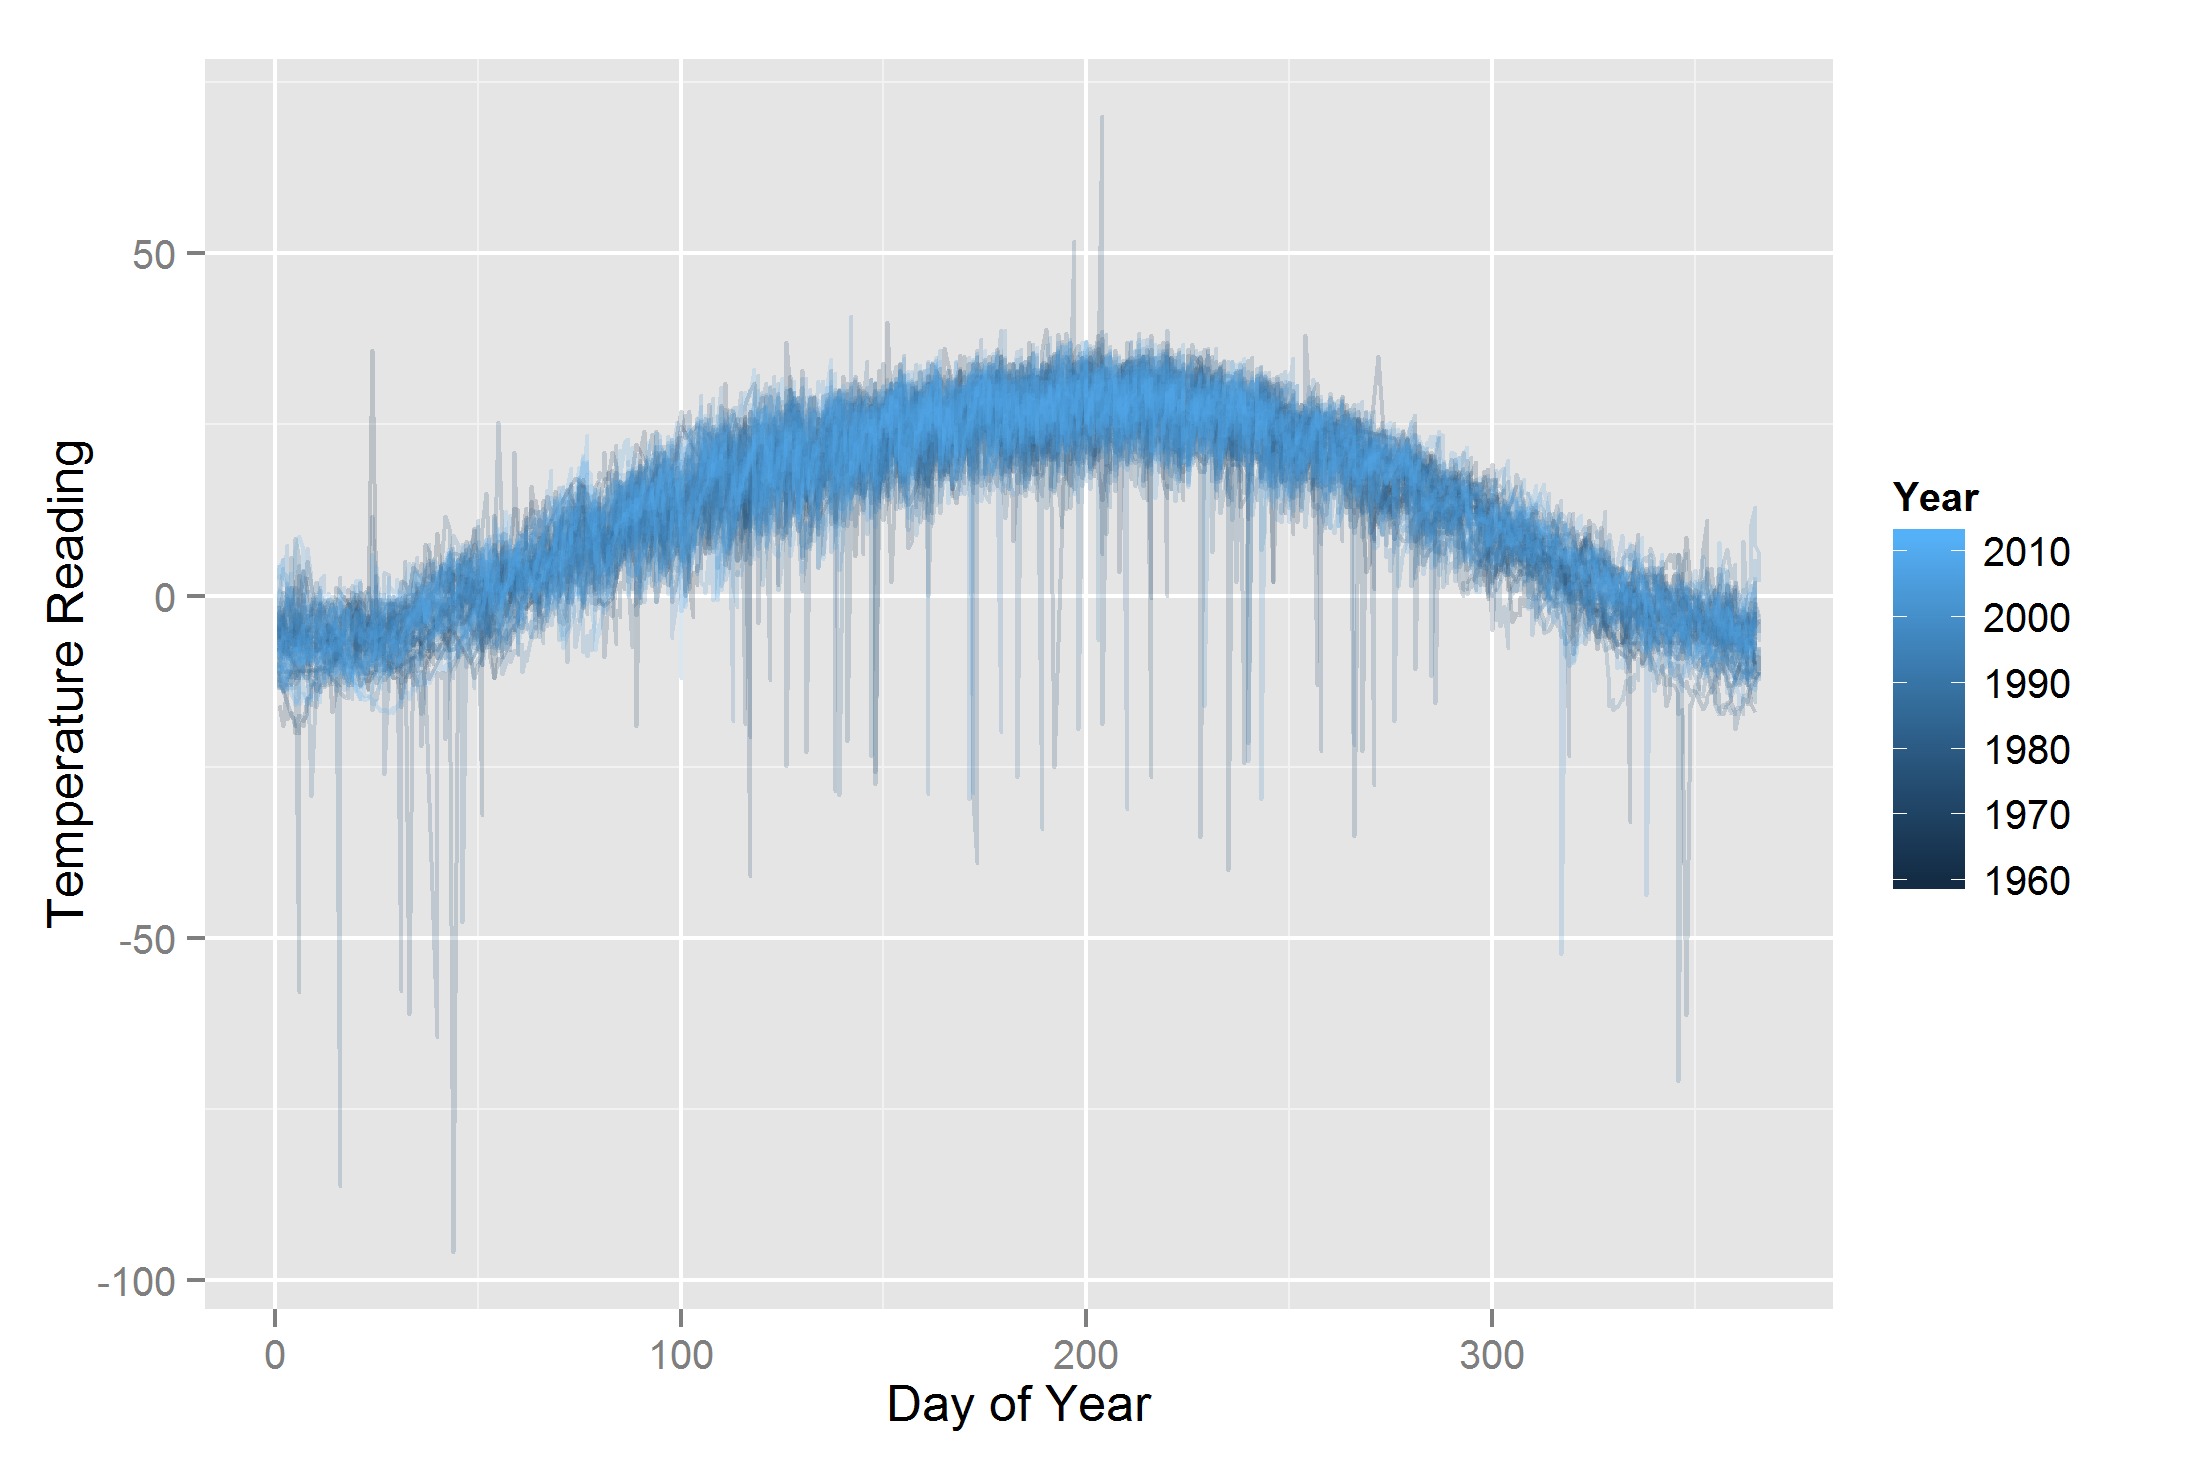
\includegraphics[width=.5\textwidth]{uadb_windc_51777_line}
		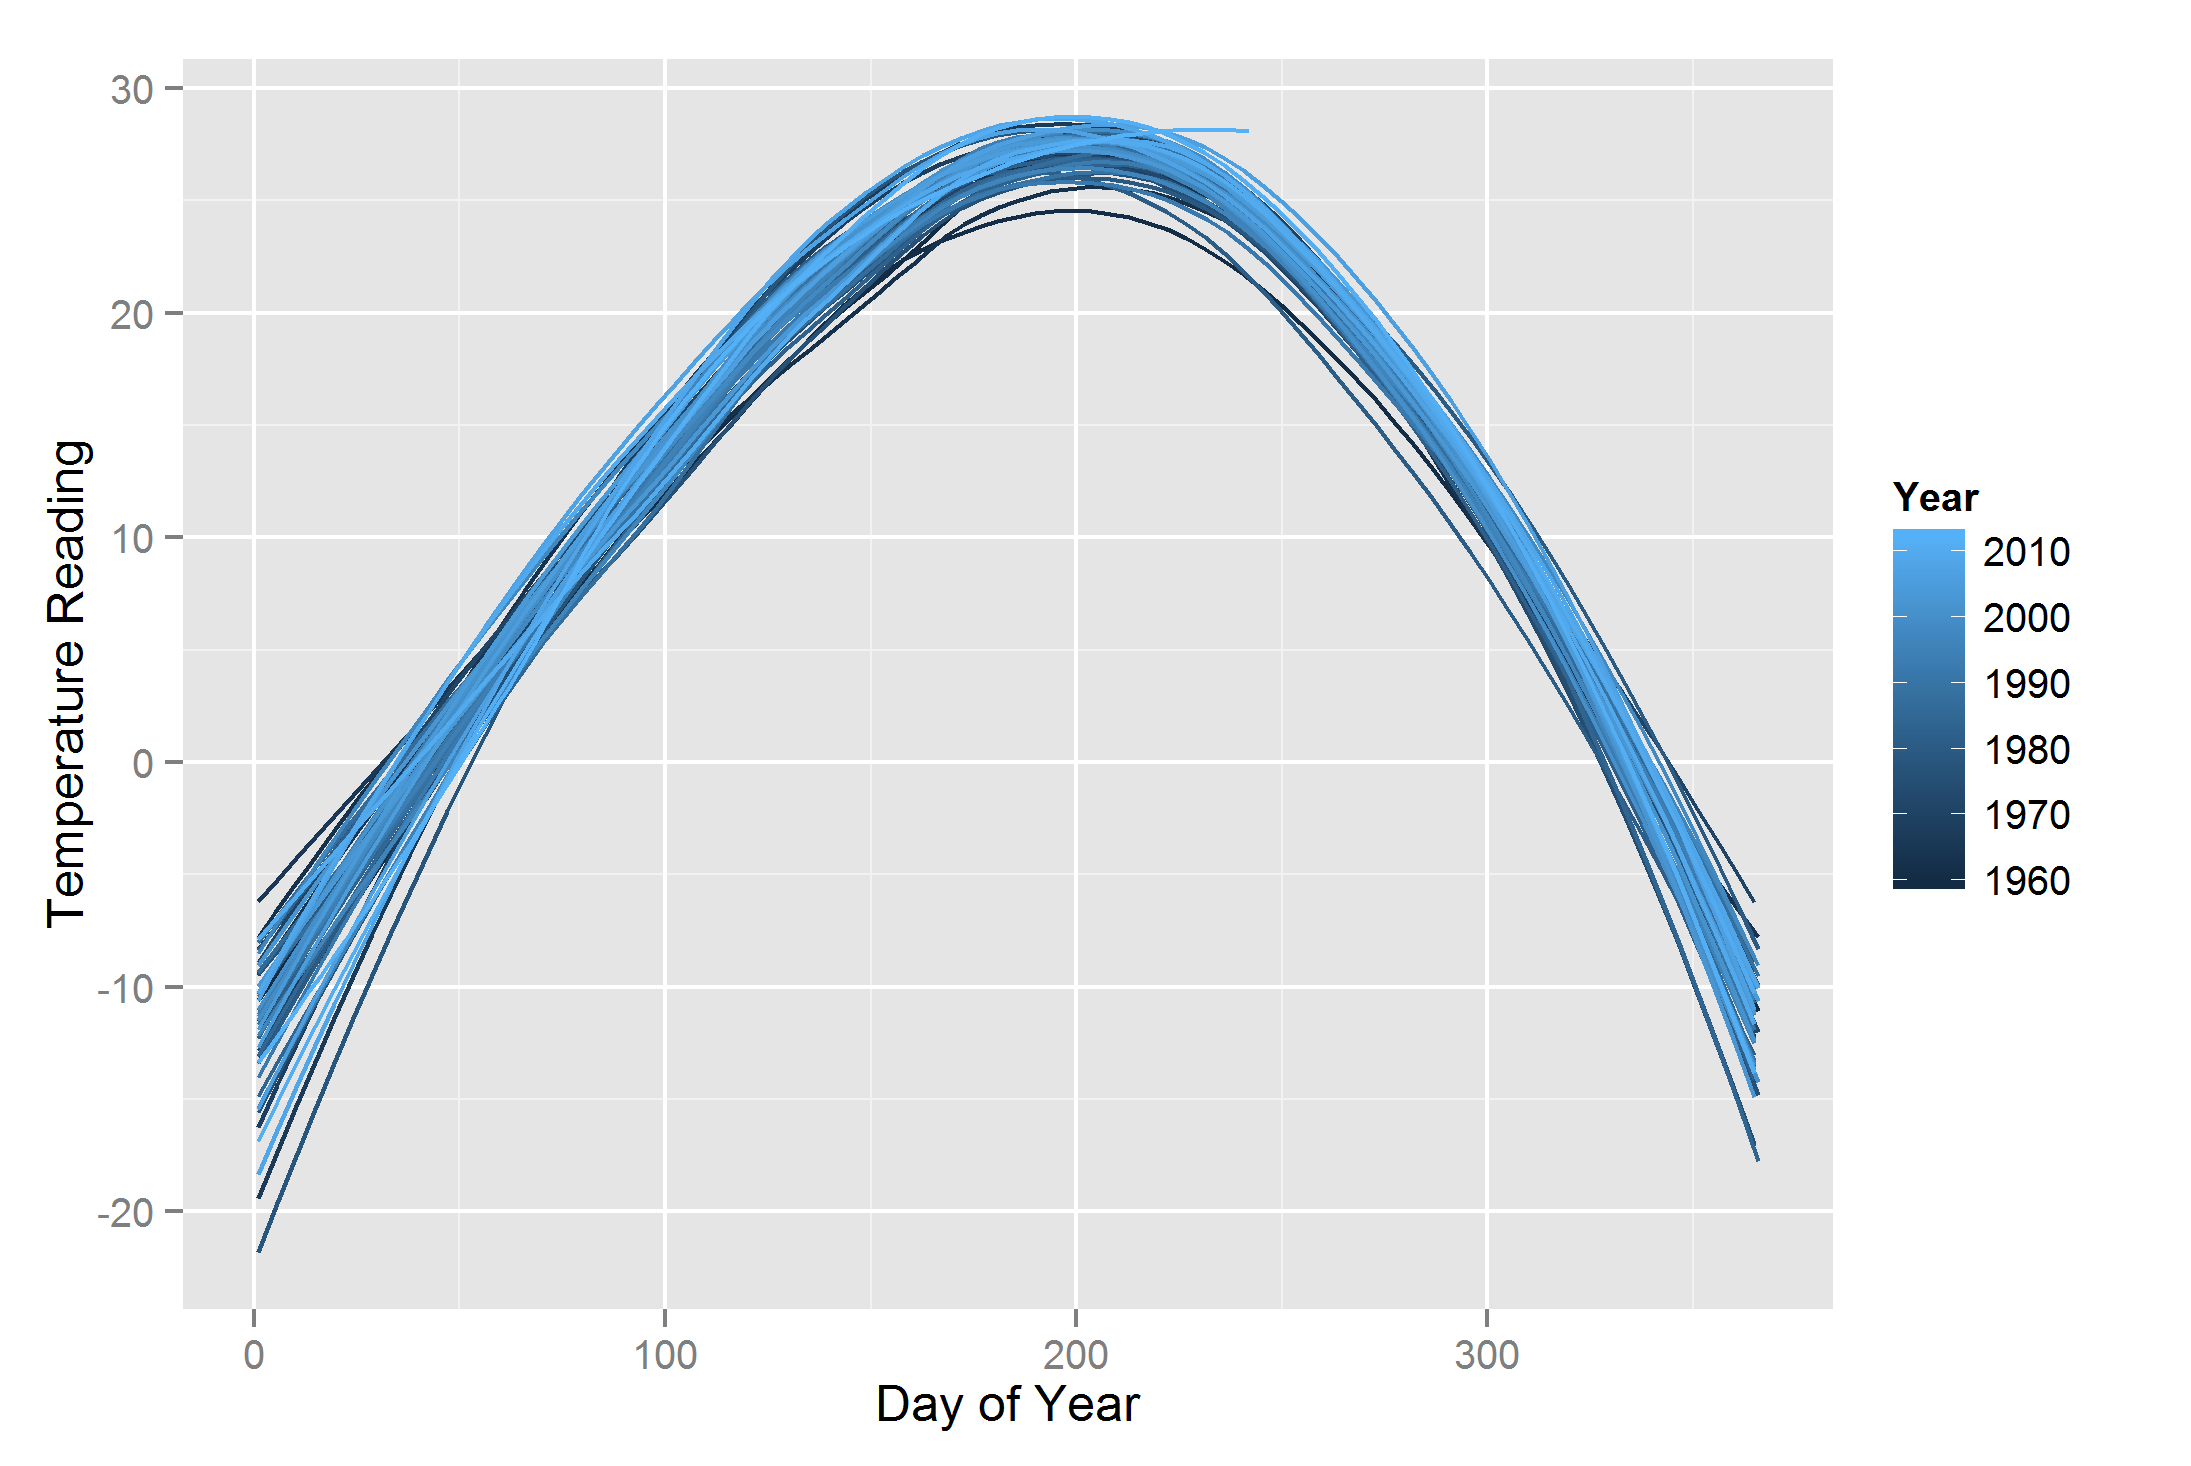
\includegraphics[width=.5\textwidth]{uadb_windc_51777_smooth}
	\end{figure}
	\begin{itemize}
		\item During the proposal, a question was raised about our data-generating model and if the seasonal trend was consistent each year.
		\item The graphs above depict the yearly time series from station 51777 (left) and a scatterplot smoother fit to each year individually (right).
	\end{itemize}
}

%\frame{\frametitle{Simulation Realizations}
%	\begin{figure}
%		\centering
%		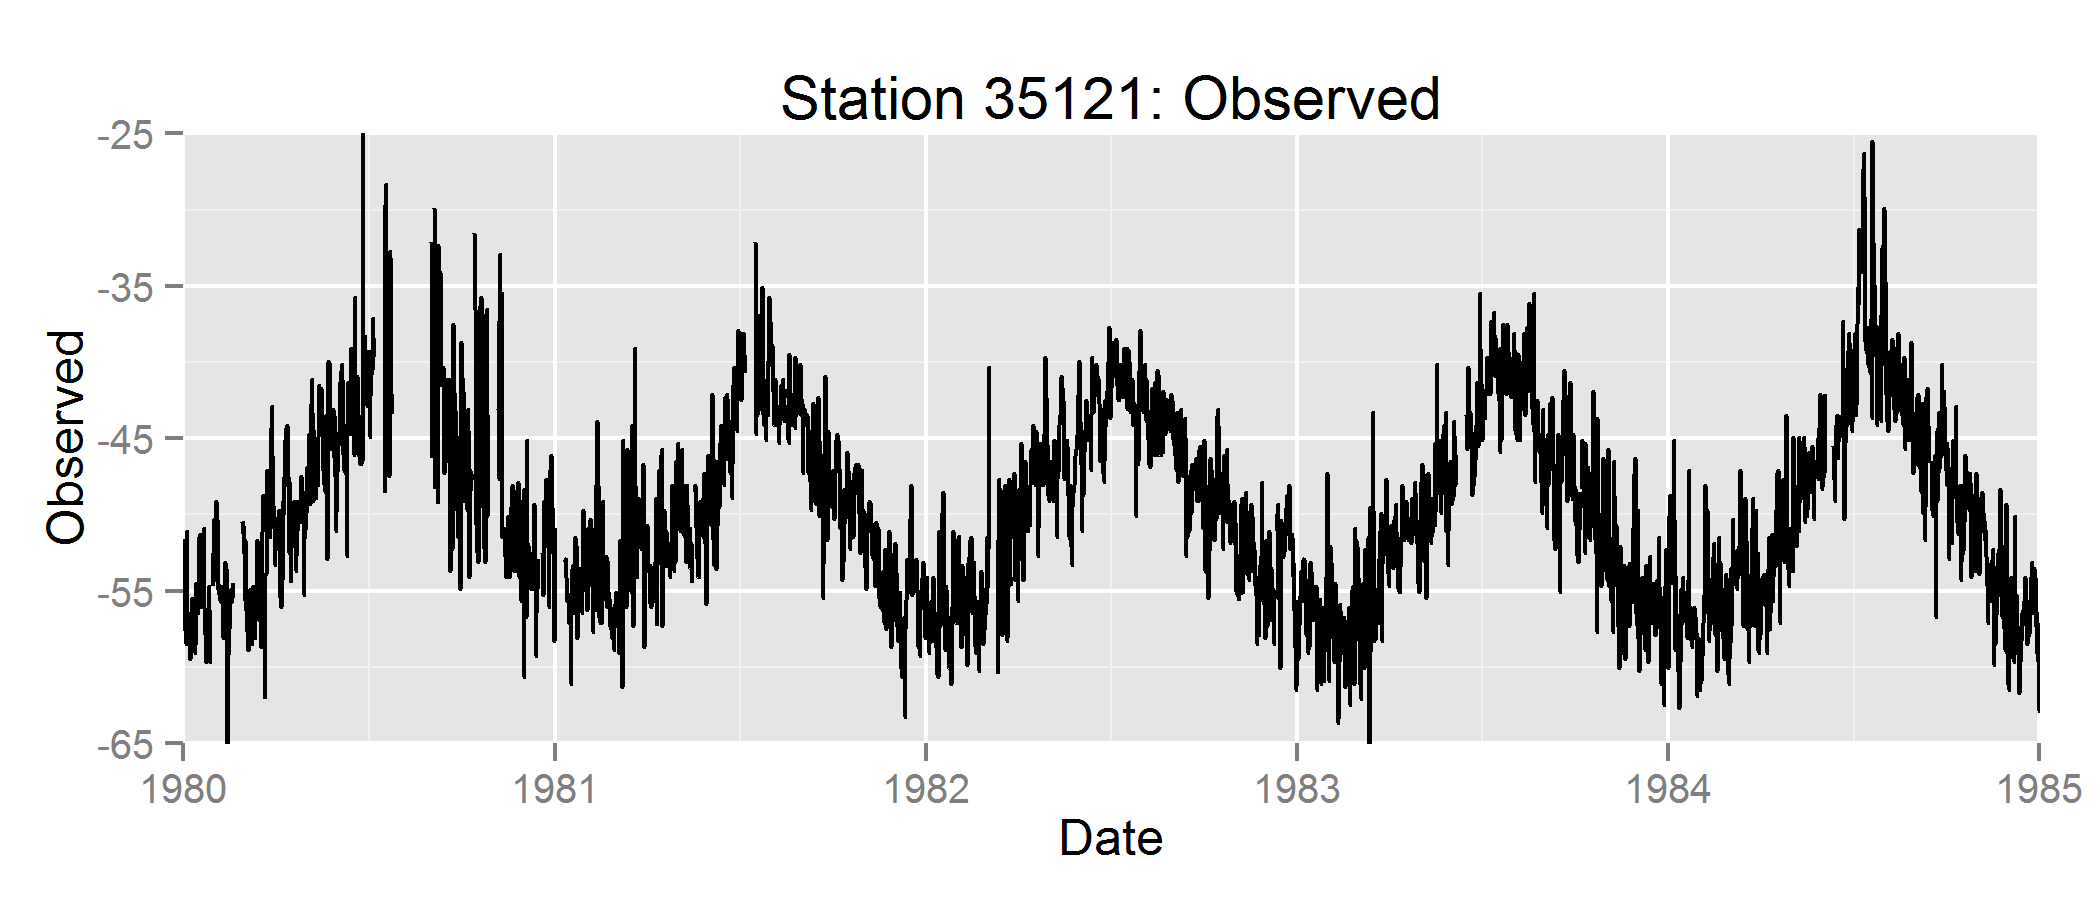
\includegraphics[width=.9\textwidth]{35121_time_series.png}\\
%		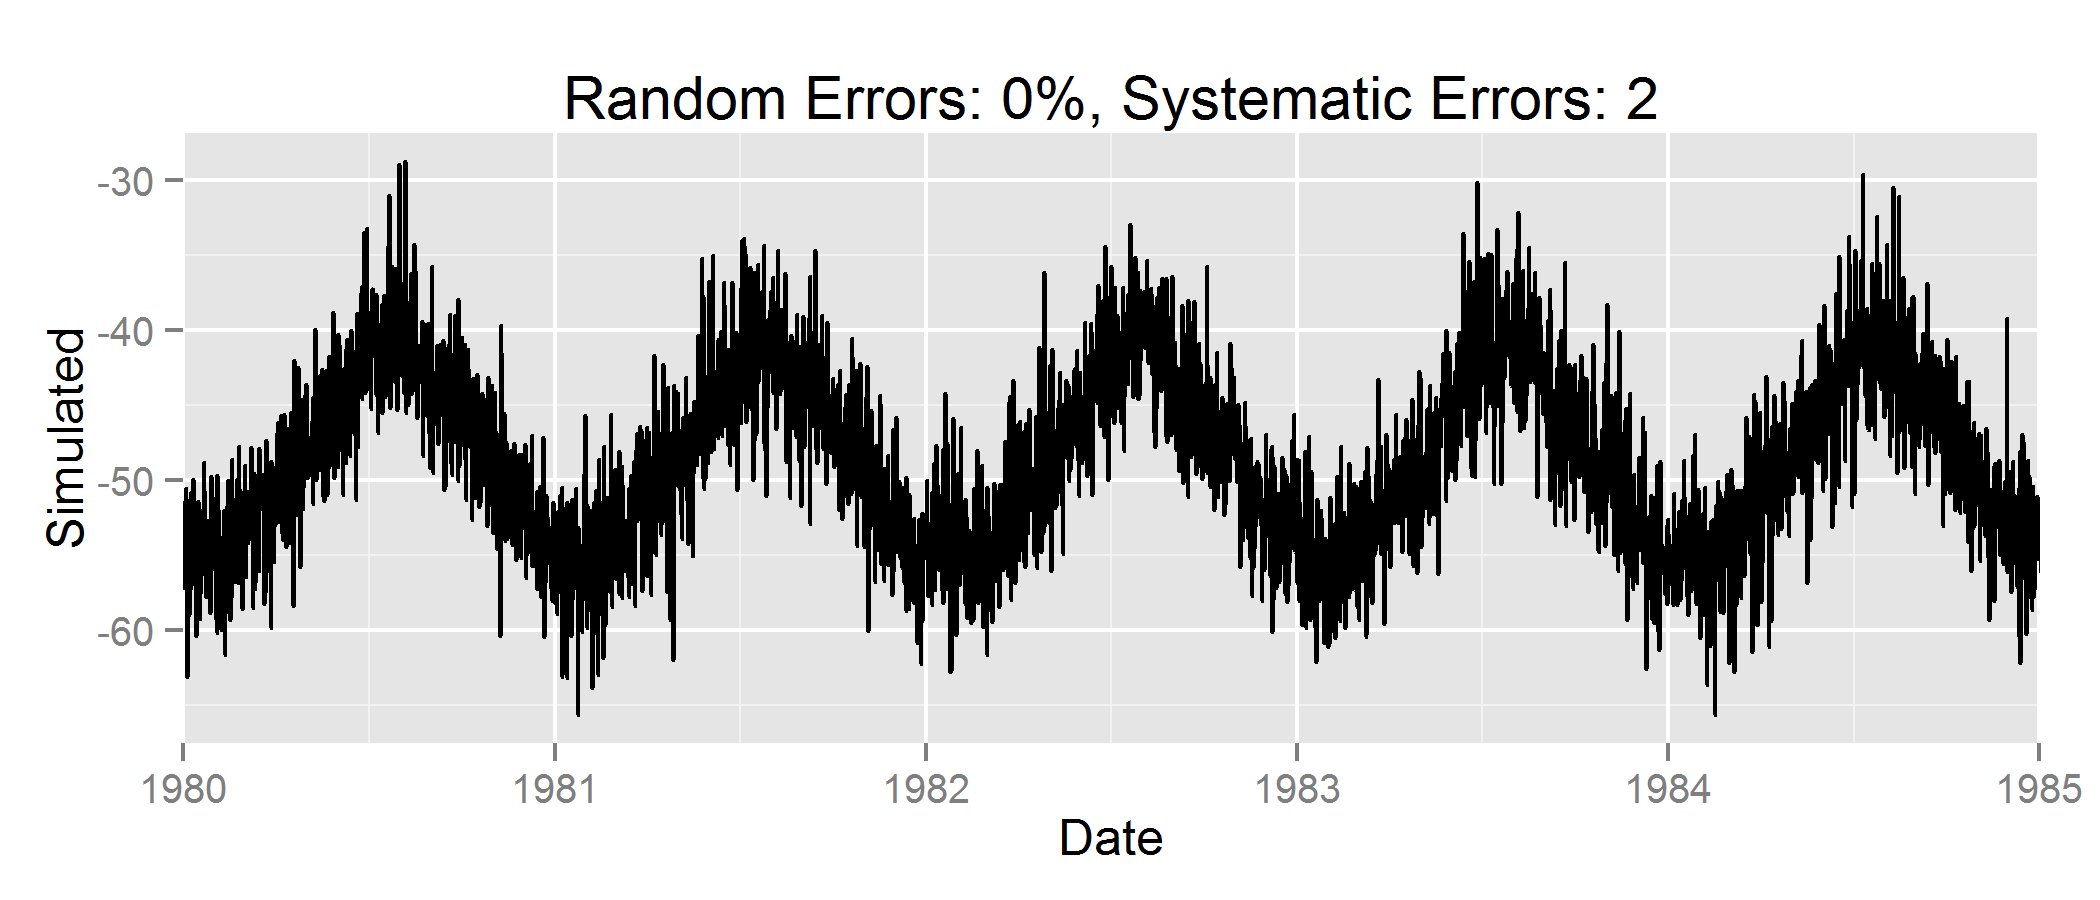
\includegraphics[width=.45\textwidth]{35121_simulated_1.png}
%		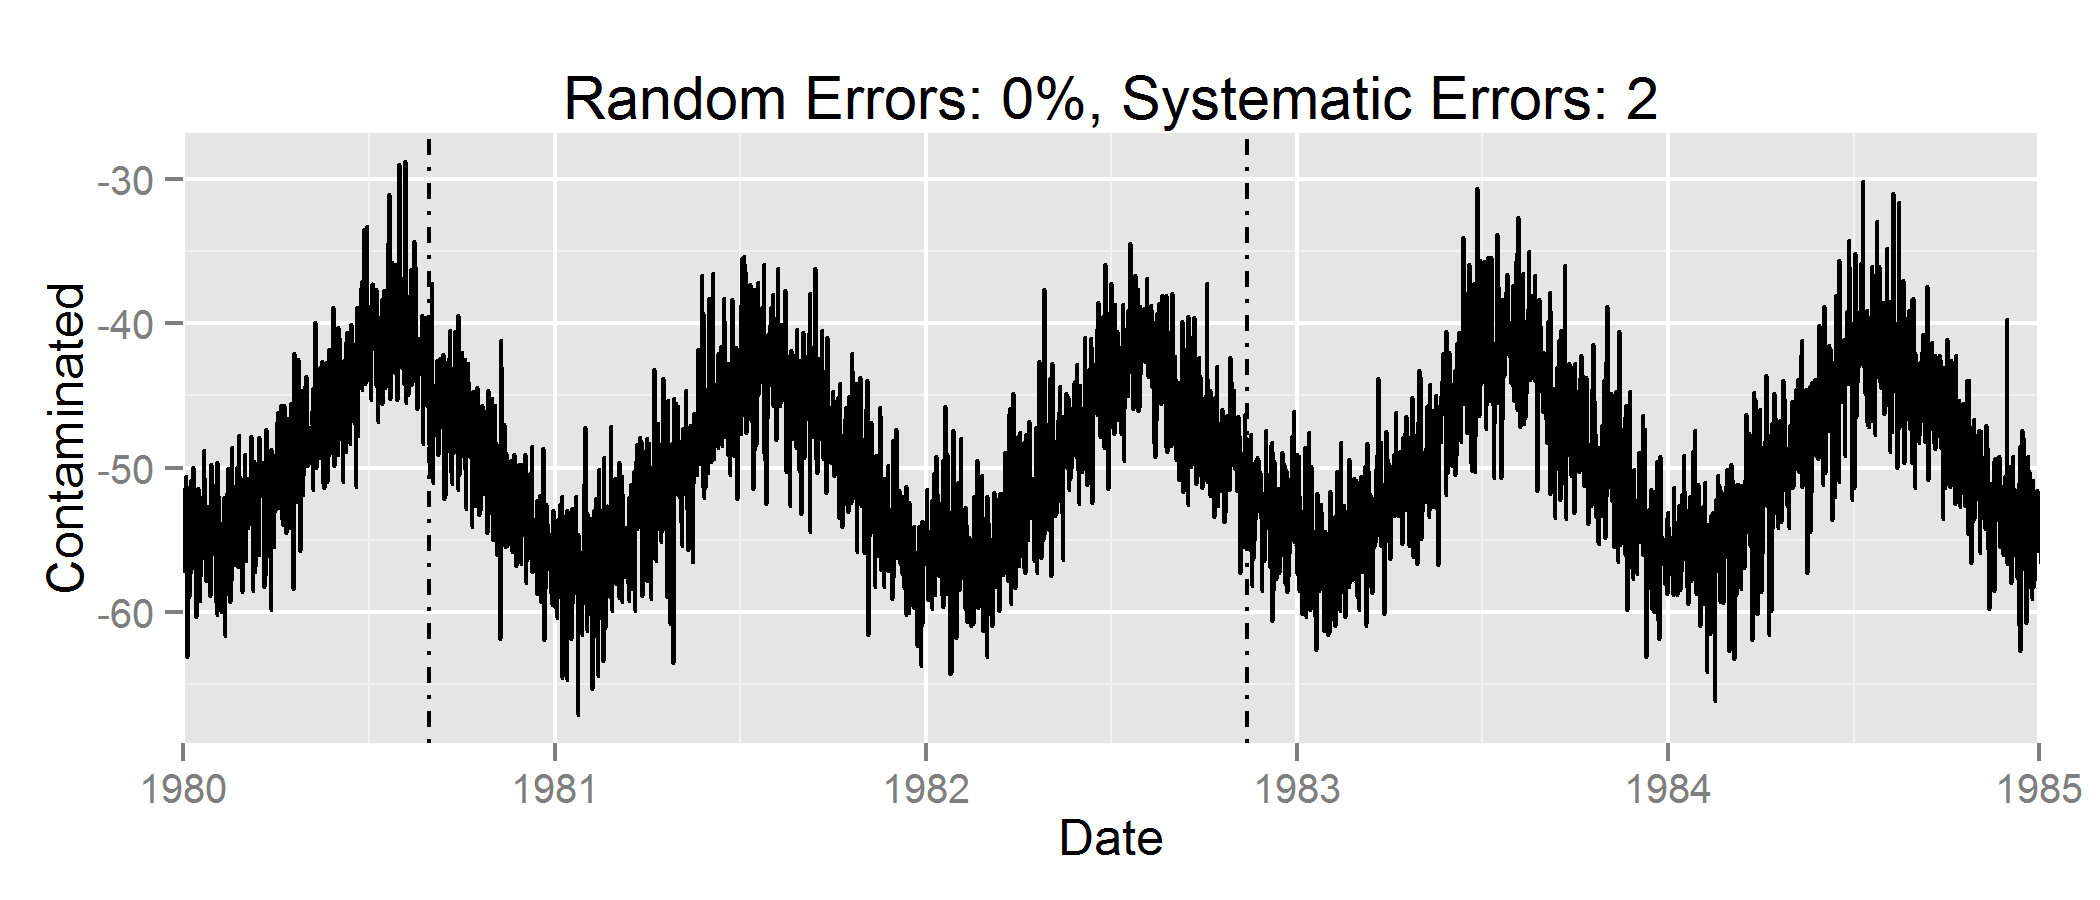
\includegraphics[width=.45\textwidth]{35121_contaminated_1.png}\\
%		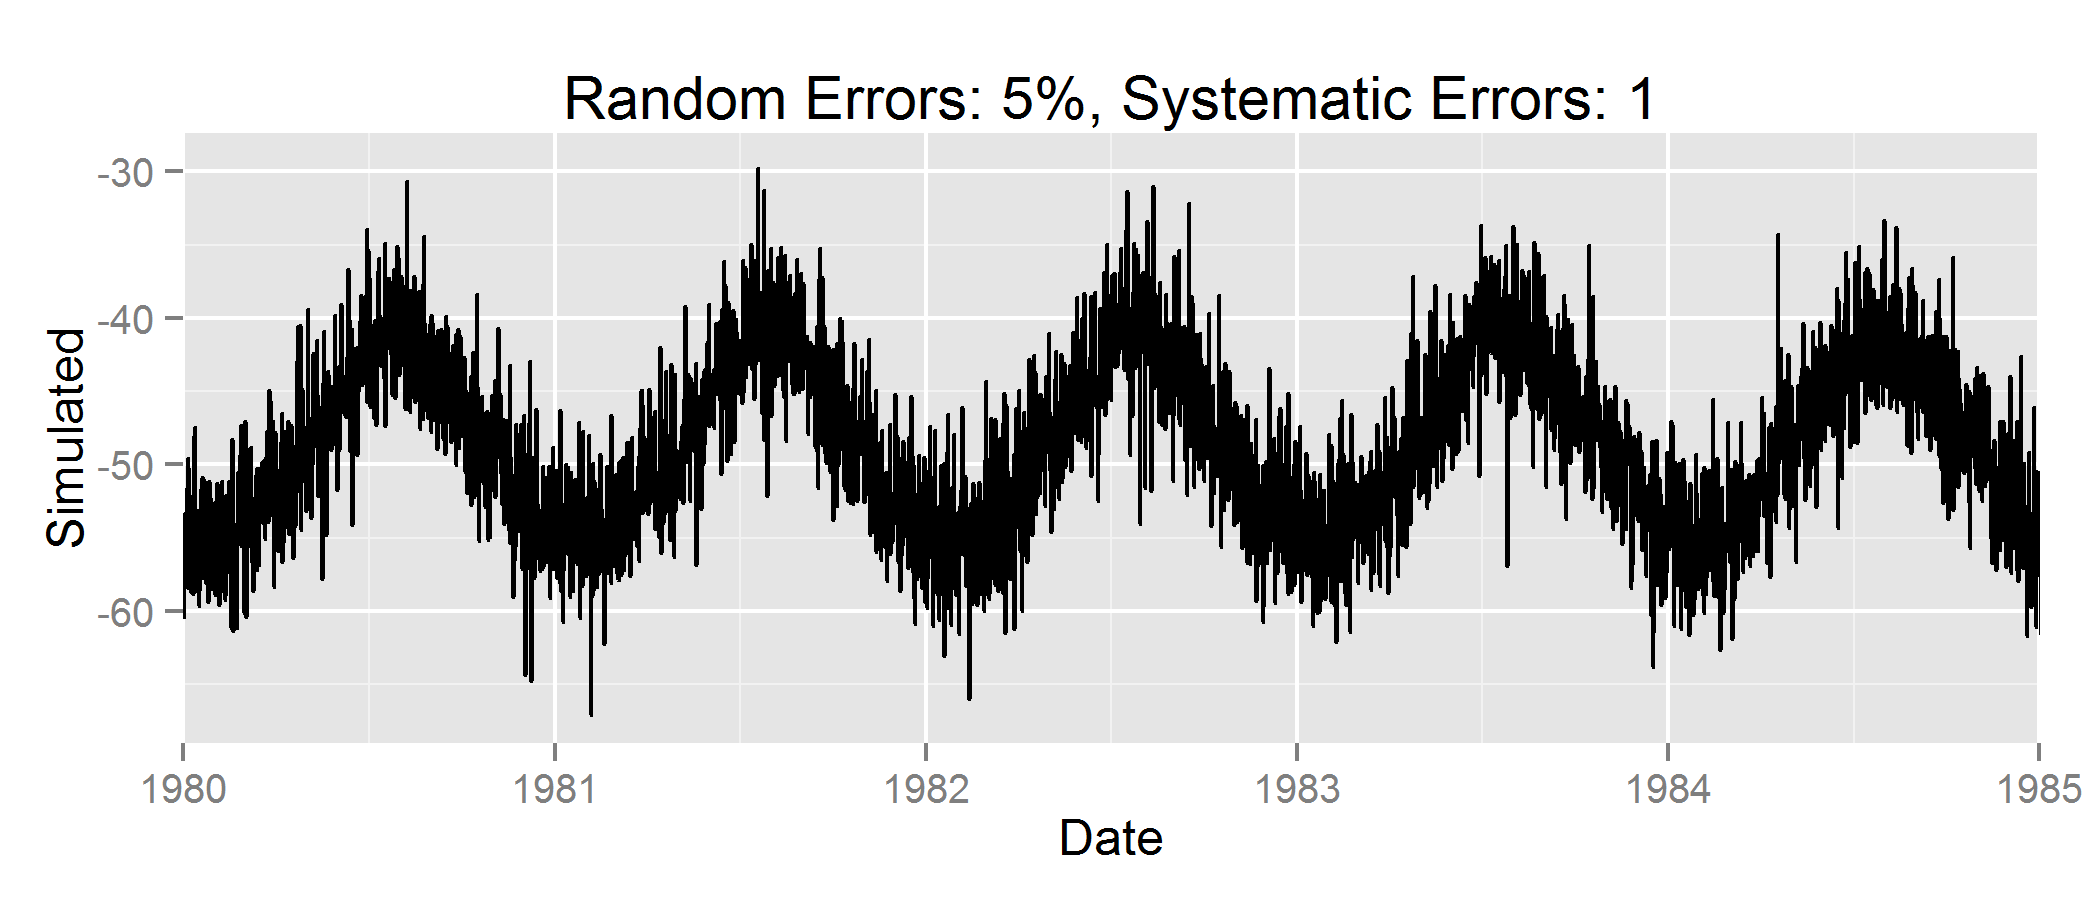
\includegraphics[width=.45\textwidth]{35121_simulated_2.png}
%		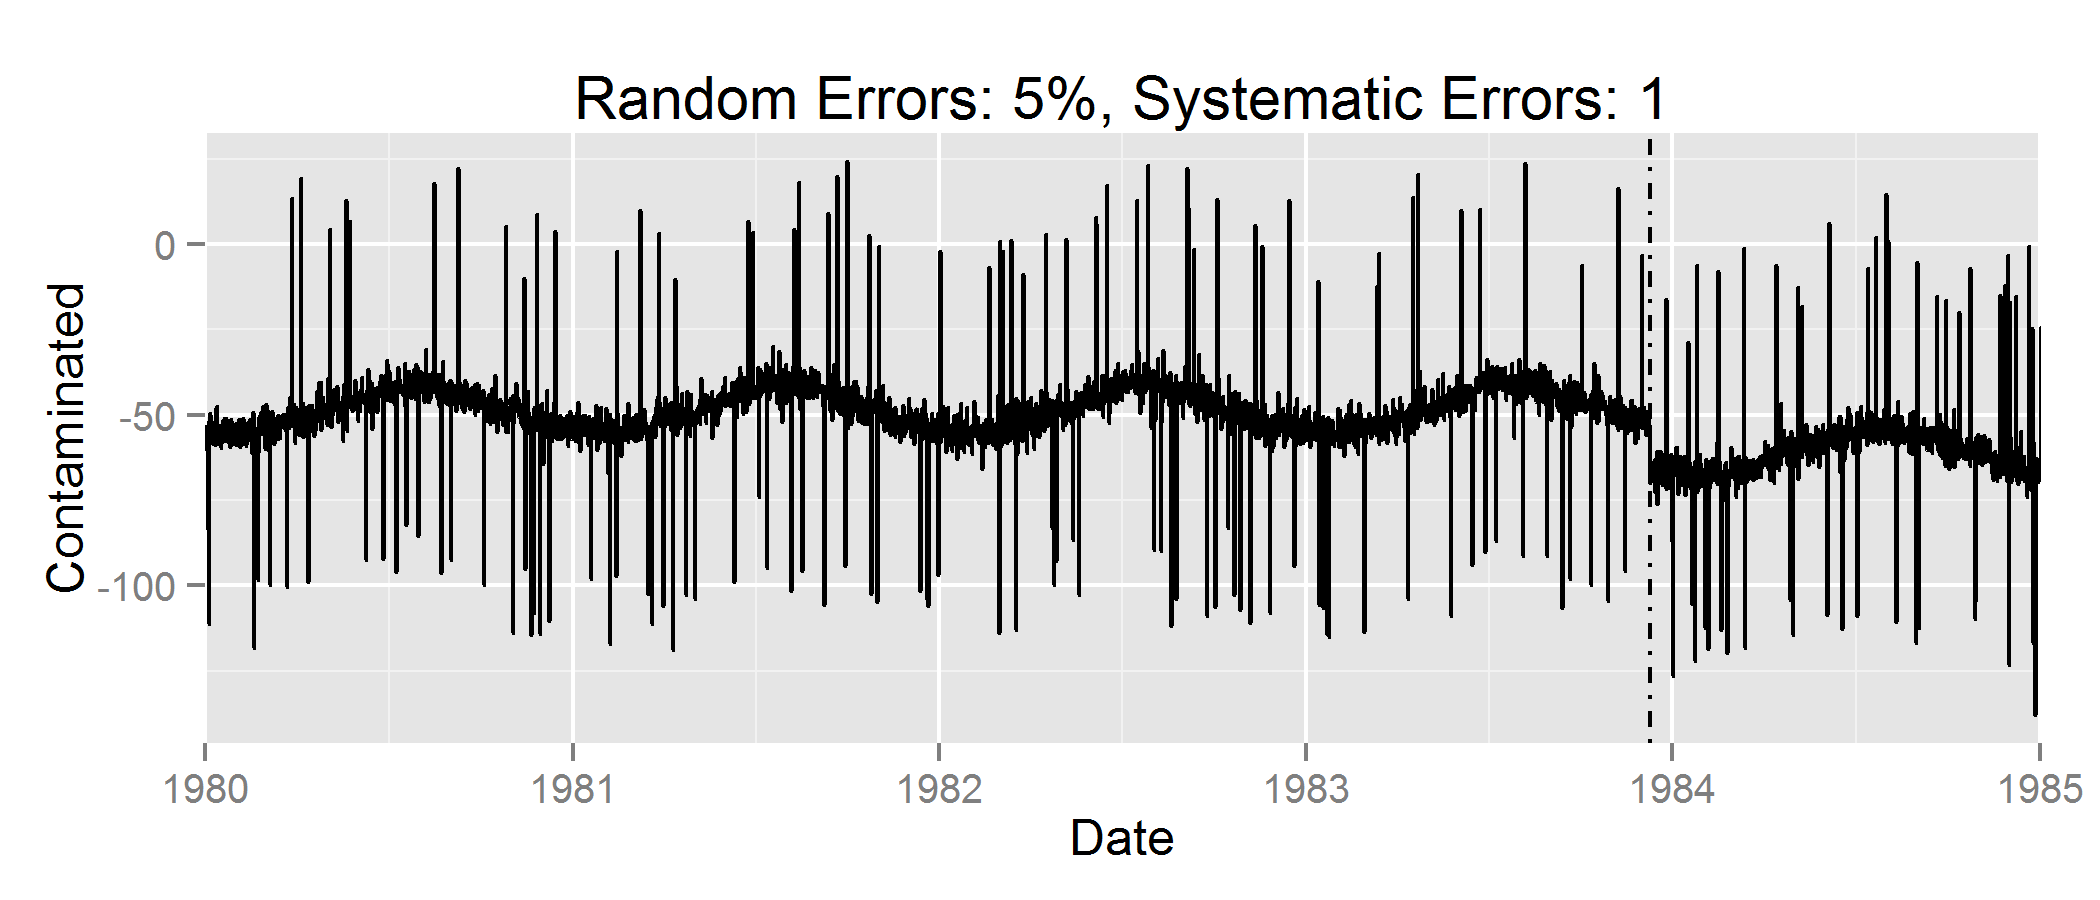
\includegraphics[width=.45\textwidth]{35121_contaminated_2.png}\\
%		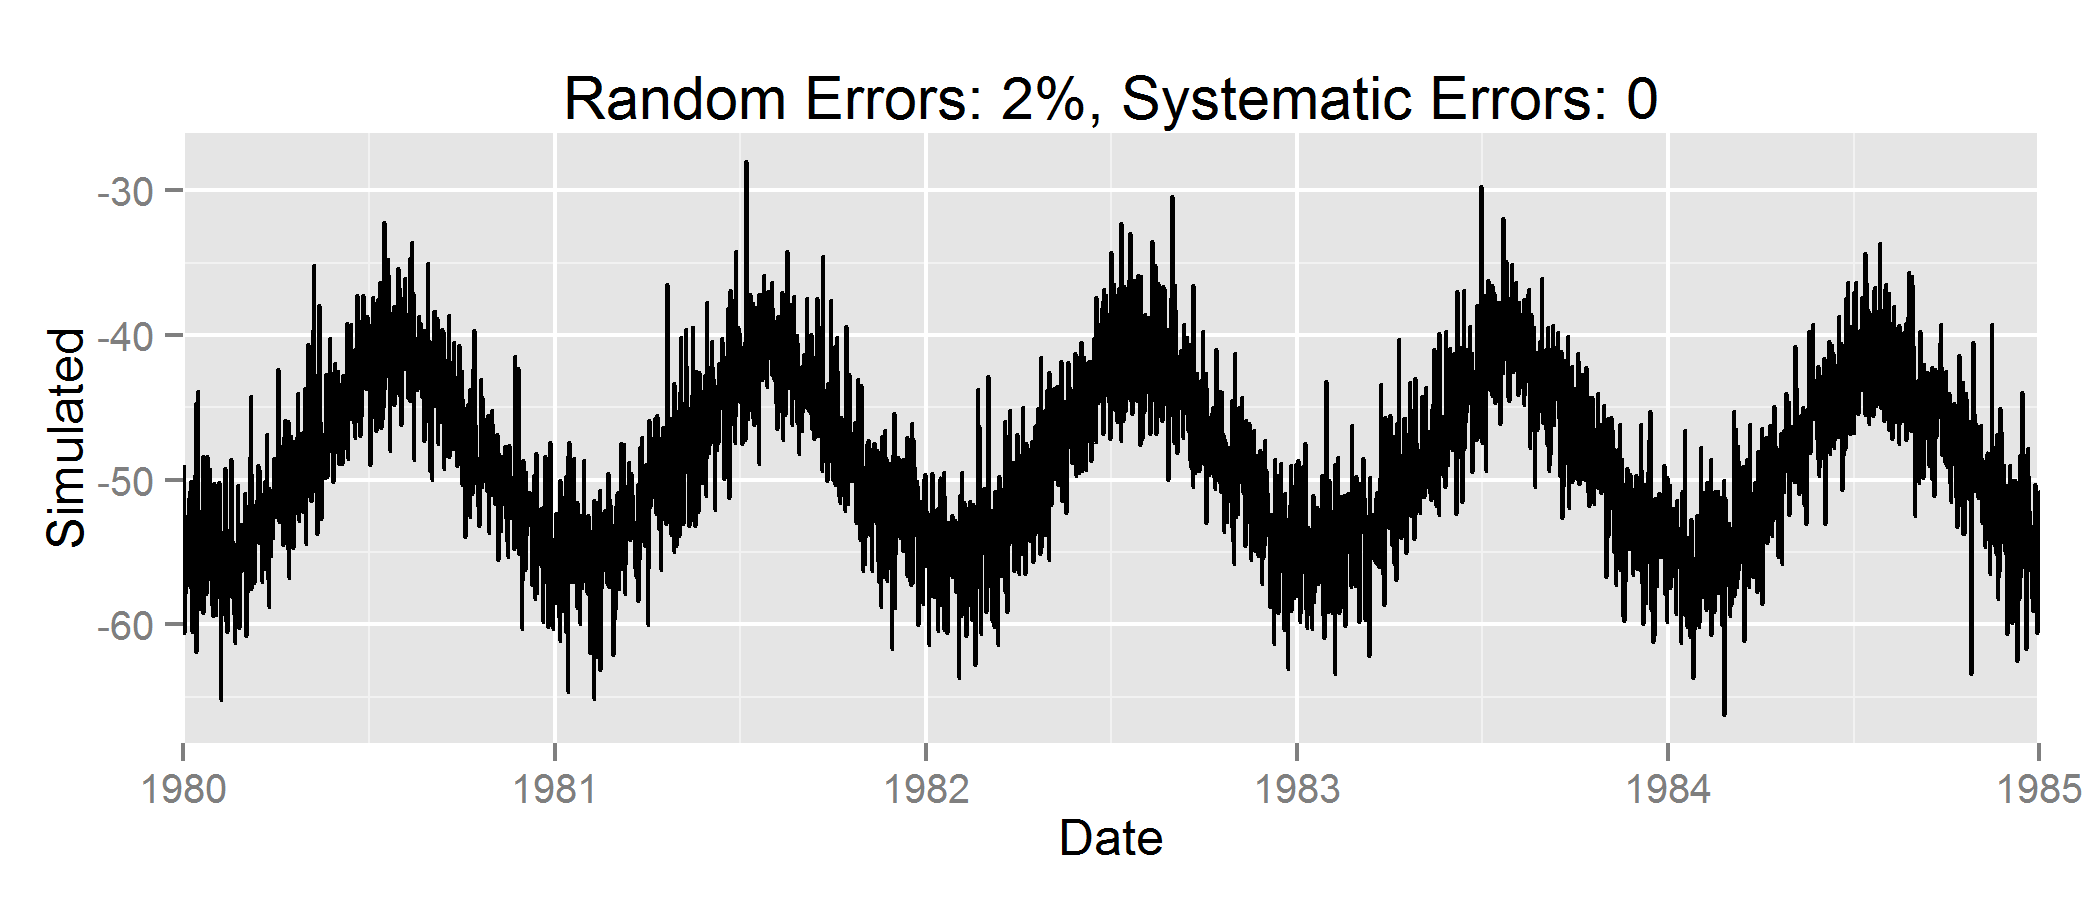
\includegraphics[width=.45\textwidth]{35121_simulated_3.png}
%		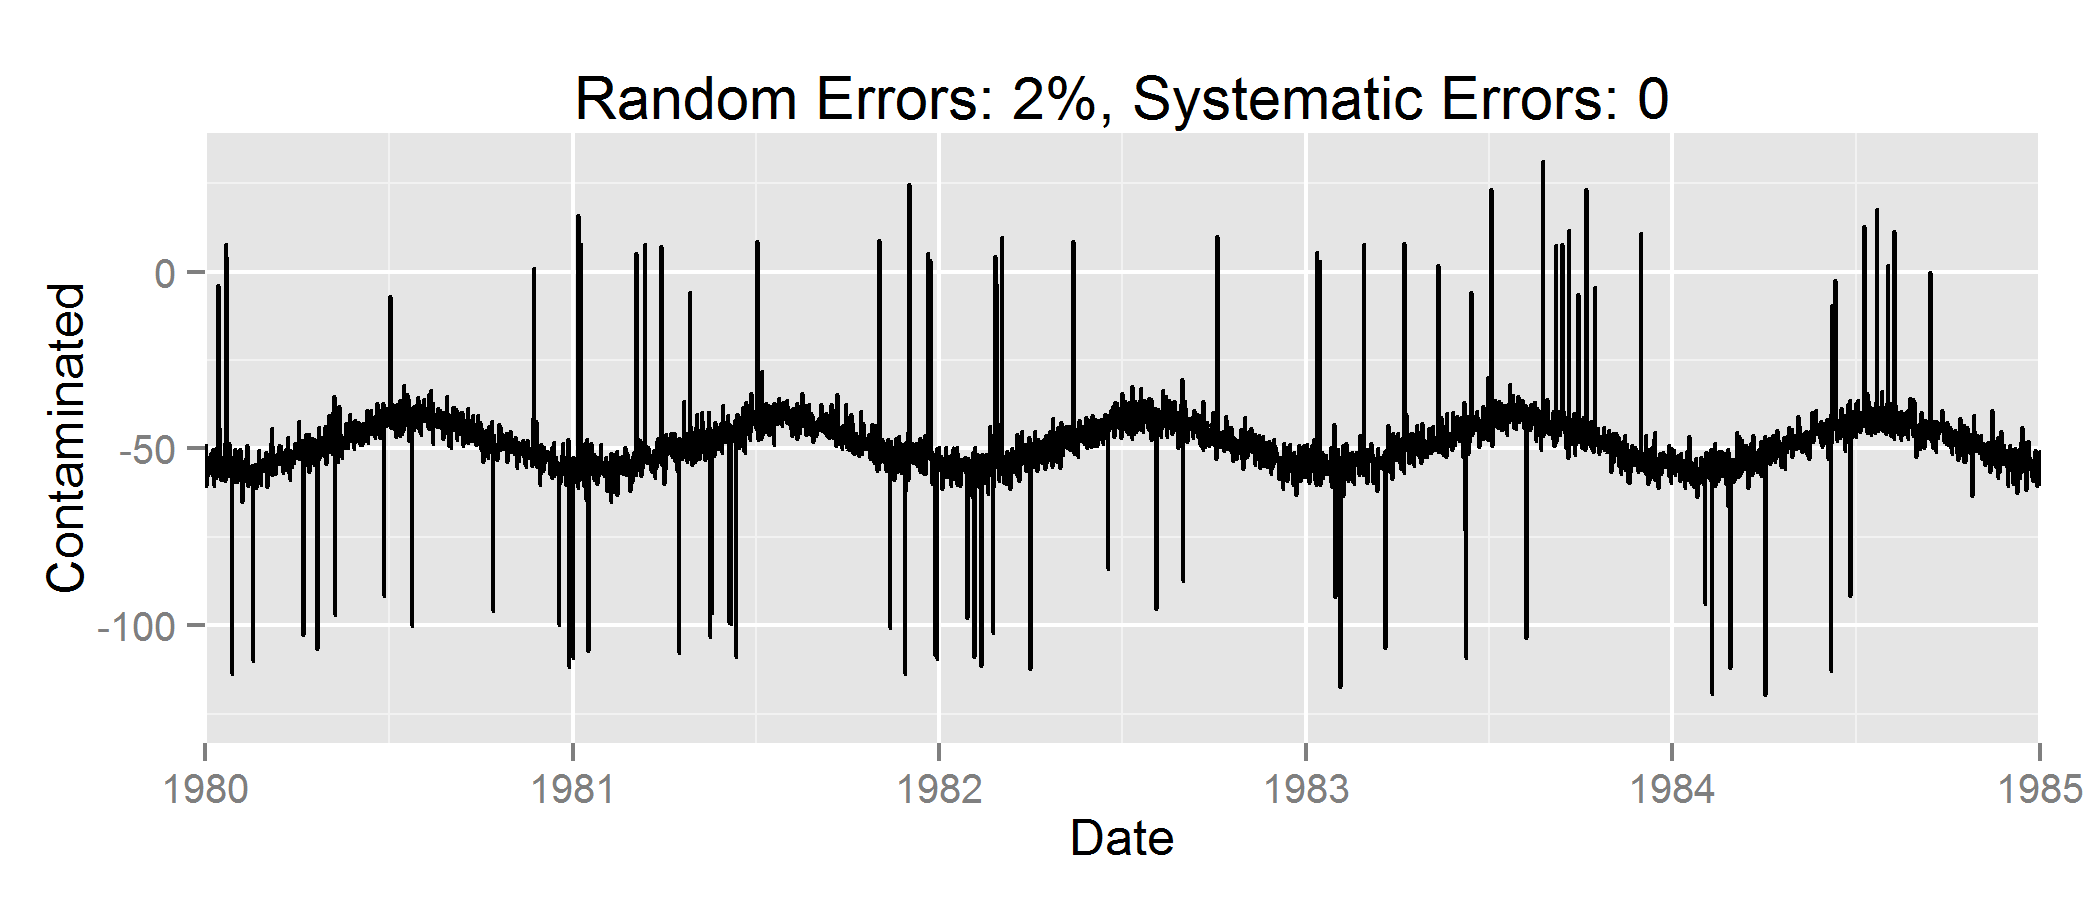
\includegraphics[width=.45\textwidth]{35121_contaminated_3.png}\\
%		\caption{Time series plots of radiosonde temperature data from station 35121.  The top plot shows the observed time series, and the following 3 pairs show three realizations of simulated datasets.  The plots on the left show the simulated data prior to contamination, and the right plots show the data after contamination with random and systematic errors.}
%		\label{fig:simExample}
%	\end{figure}
%}

\subsection{Performance Metrics}

\frame{\frametitle{Performance Metrics}
	\small
	\begin{itemize}
		\item \textbf{True Positive Rate:}  The proportion of simulated errors correctly detected by the quality control algorithm.
		\item \textbf{False Positive Rate:}  The proportion of valid data points incorrectly identified as errors by the quality control algorithm.
		\item \textbf{Efficiency:}  Let $\mathbf{x}$, $\mathbf{c}$, and $\mathbf{h}$ be the original, contaminated, and contaminated and homogenized time series, respectively and let the $i$-th observation be denoted by $x_i, c_i$, and $h_i$ respectively.  The Root Mean Square Error (RMSE) of $\mathbf{h}$ is then defined as follows:
		\begin{equation*}
		\mbox{RMSE}(\mathbf{h}) = \sqrt{\frac{1}{n} \sum_{i=1}^n (h_i-x_i)^2}.
		\end{equation*}
		Then, the efficiency of the homogenized series, where 1 means perfect skill, 0 means no improvement, and negative values indicate degradation is
		\begin{equation*}
		\mbox{Eff}(\mathbf{h}) = \frac{\mbox{RMSE}(\mathbf{c})-\mbox{RMSE}(\mathbf{h})}{\mbox{RMSE}(\mathbf{c})}.
		\end{equation*}
	\end{itemize}
}

\section{Results}

\subsection{Homogenization Algorithms}

\frame{\frametitle{Tuning Parameters}
	\begin{itemize}
		\item PELT: The cost function for PELT and BinSeg allow for an increase in the penalty as a function of the number of change points.  Thus, I consider penalties of $\beta=n/2$, $n$, $2n$, $4n$, and  $8n$.
		\item BinSeg: I use no penalty term and instead restrict the maximum number of change points that can occur, varying from 1 to 10.
		\item SNHT: This algorithm computes means of seasonal data, so periods which are multiples of a year should be considered.  Thus, I use one and two year averaging windows with $N=365$ or $N=730$.
		\item Robust SNHT: I use $N=365$ and $N= 730$.
	\end{itemize}
}

\frame{\frametitle{Observed Efficiencies}
\small
\vspace{-0.2cm}
\begin{figure}
	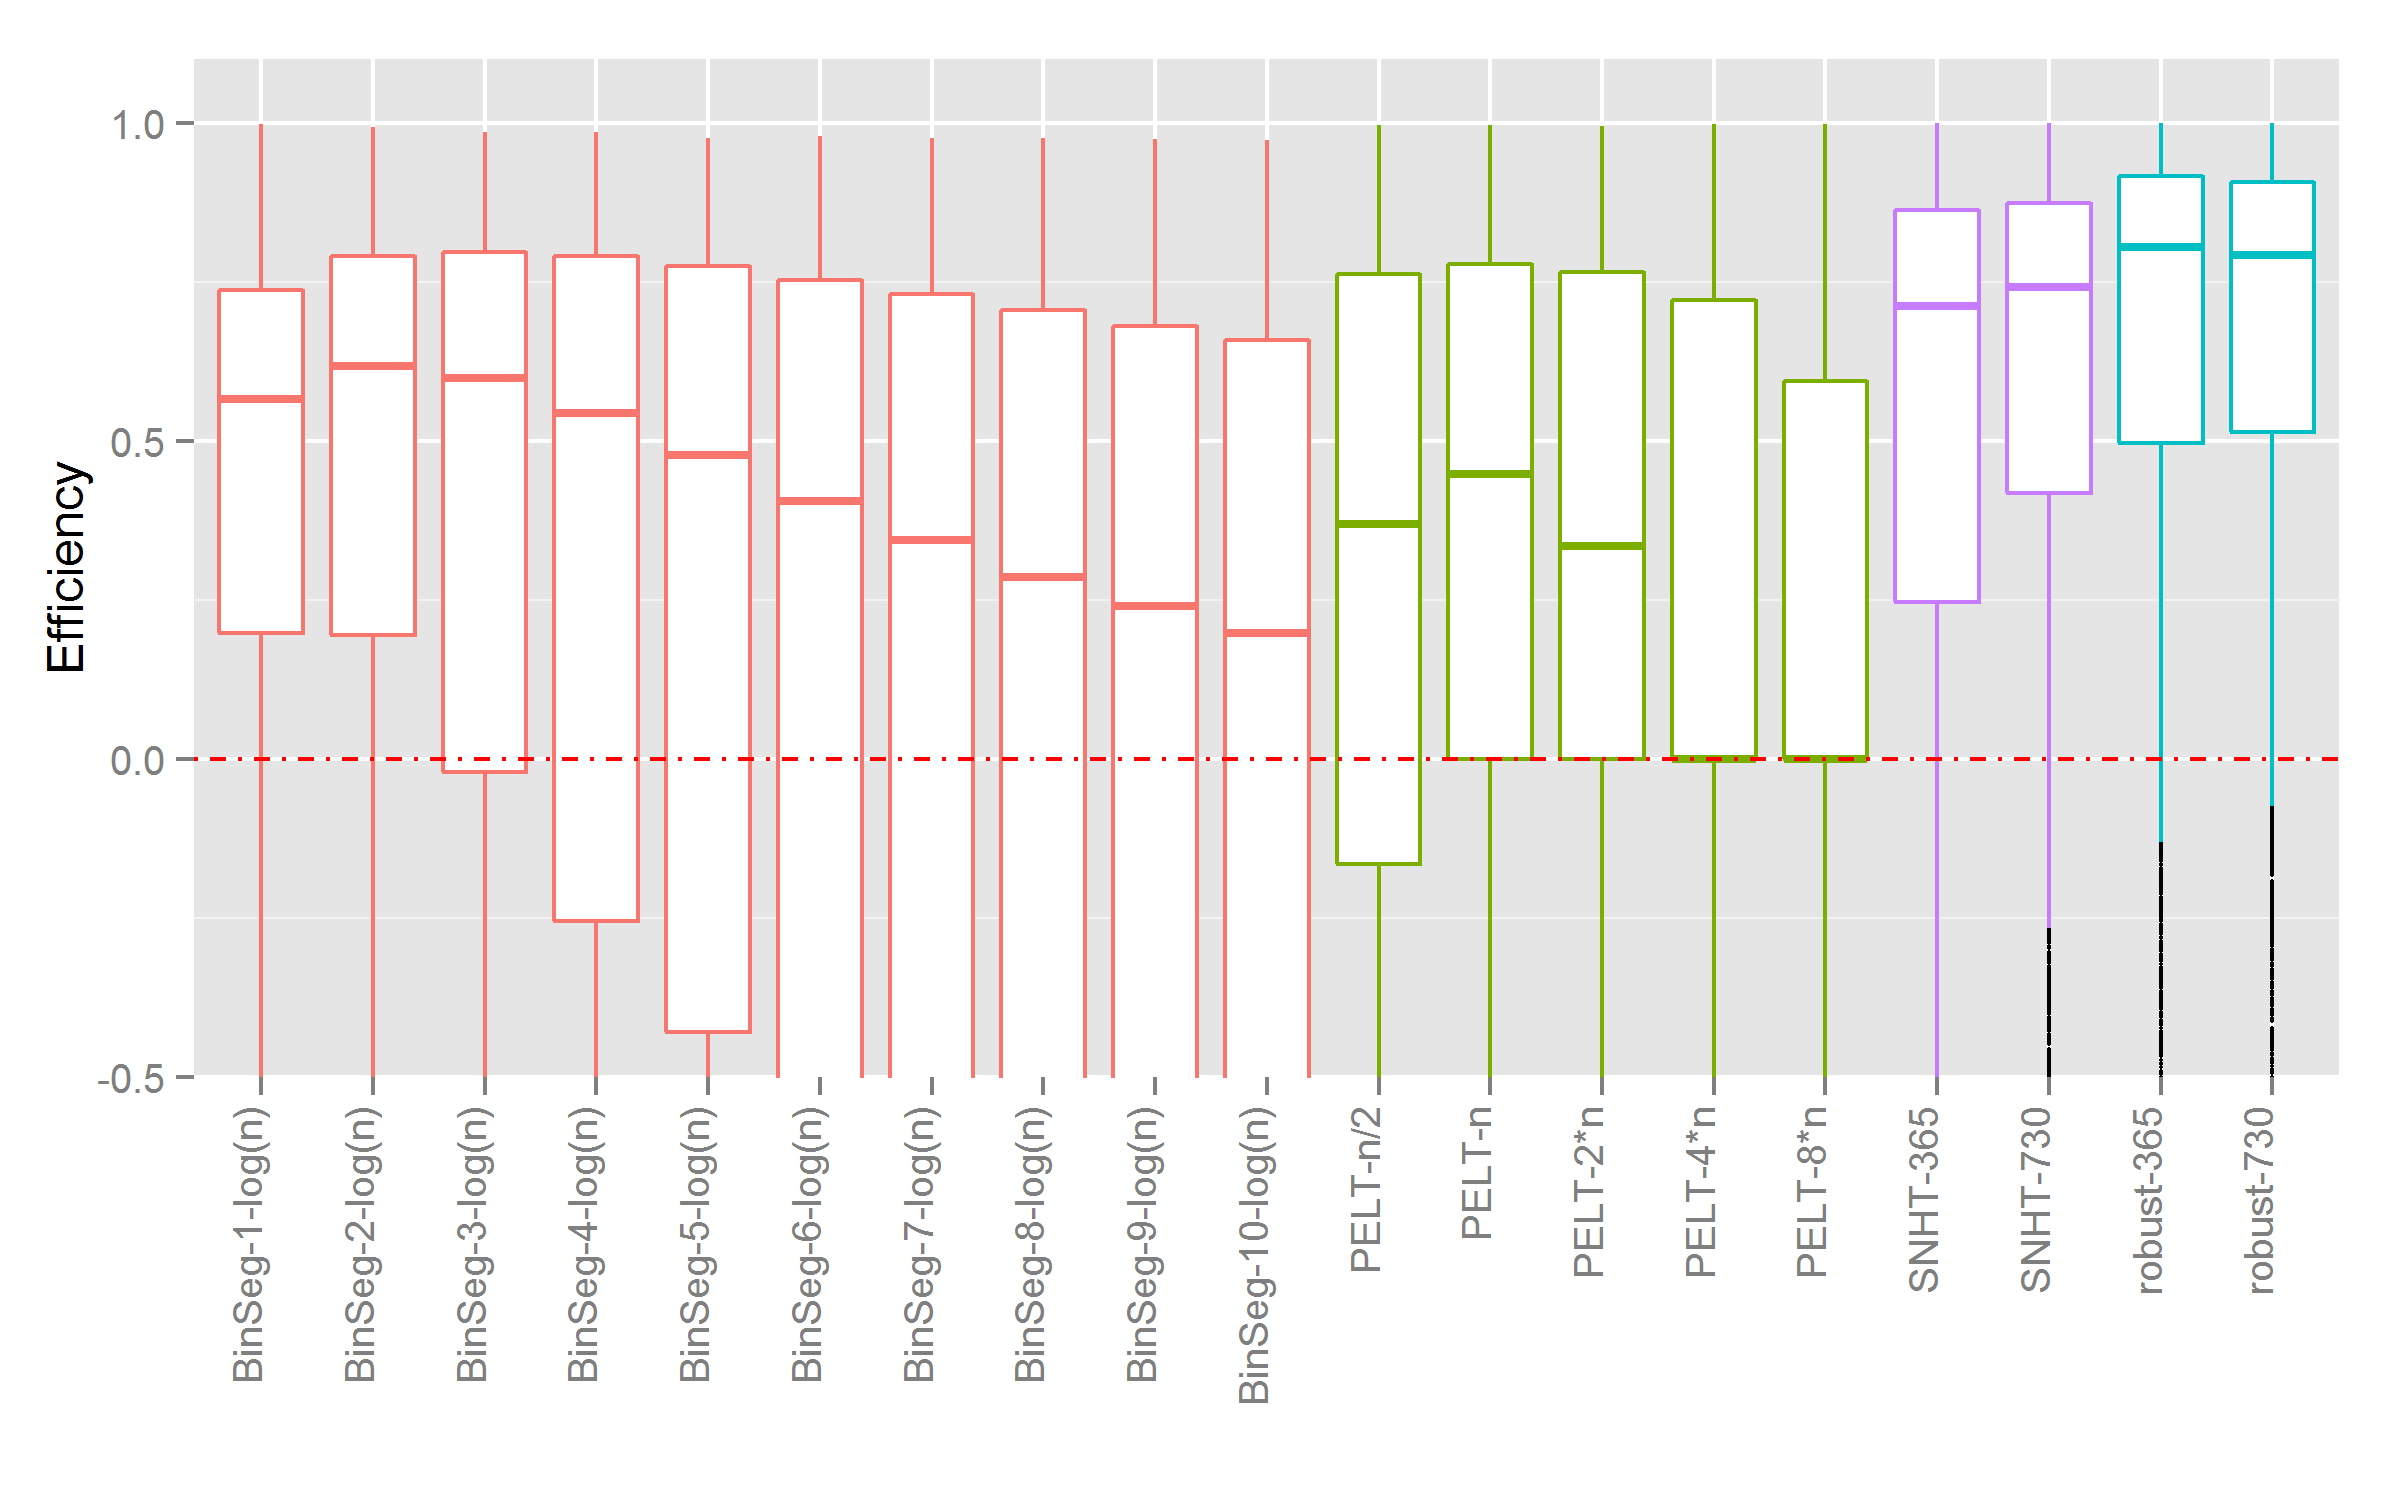
\includegraphics[width=.8\textwidth]{Efficiency_Model_Plot}
\end{figure}
\vspace{-0.5cm}
\begin{itemize}
	\item This plot depicts the observed efficiencies for the various homogenization algorithms.
	\item Most algorithms tend to have efficiencies above 0, but some of the BinSeg algorithms substantially overfit.
	\item This graph suggests that the SNHT and robust SNHT attain the highest efficiency, and that the robust version is slightly better than the traditional.
\end{itemize}
}

\frame{\frametitle{Logistic Regression Model Selection}
\begin{itemize}
	\item In order to analyze the results more effectively, and to understand the influence of different simulation parameters, I fit a logistic regression model to the results.  Let $Y_i$ be the probability that the efficiency is greater than 0 for the $i$th simulation, then
	$$Y_i \sim \mbox{Bernoulli}(0,p_i), \hspace{1cm} g(p_i)=X_{i\cdot} \beta$$
	where
	\begin{itemize}
		\small
		\item $g(\cdot)$ is the logit link
		\item $X$ is my design matrix consisting of sample size, outlier contamination rate, station, pressure, and homogenization algorithm.
		\item $\bbeta$ is a vector of the estimated coefficients
	\end{itemize}
\end{itemize}
}

\frame{\frametitle{Logistic Regression Model Selection}
\begin{itemize}
	\item I allowed for interaction effects, and considered models with only main effects up to models with all 5-way interactions.
	\item I used the deviance of these different models to assess model fit and choose which model to interpret.
\end{itemize}
\begin{table}[ht]
	\centering
	\begin{tabular}{lcc}
		\hline
		Model Type & Deviance & \% Reduction\\
		\hline
		Intercept Only & 672836 & ---\\ 
		Main Effects & 529612 & 21.29\%\\ 
		\textbf{2-Way Interactions} & \textbf{501158} & \textbf{5.37}\%\\ 
		3-Way Interactions & 490553 & 2.12\% \\ 
		4-Way Interactions & 487125 & 0.70\% \\ 
		5-Way Interactions & 486493 & 0.13\% \\ 
		\hline
	\end{tabular}
	\label{tab:homOrdDev}
\end{table}
}

\frame{\frametitle{Logistic Regression Model Coefficients}
\begin{figure}
	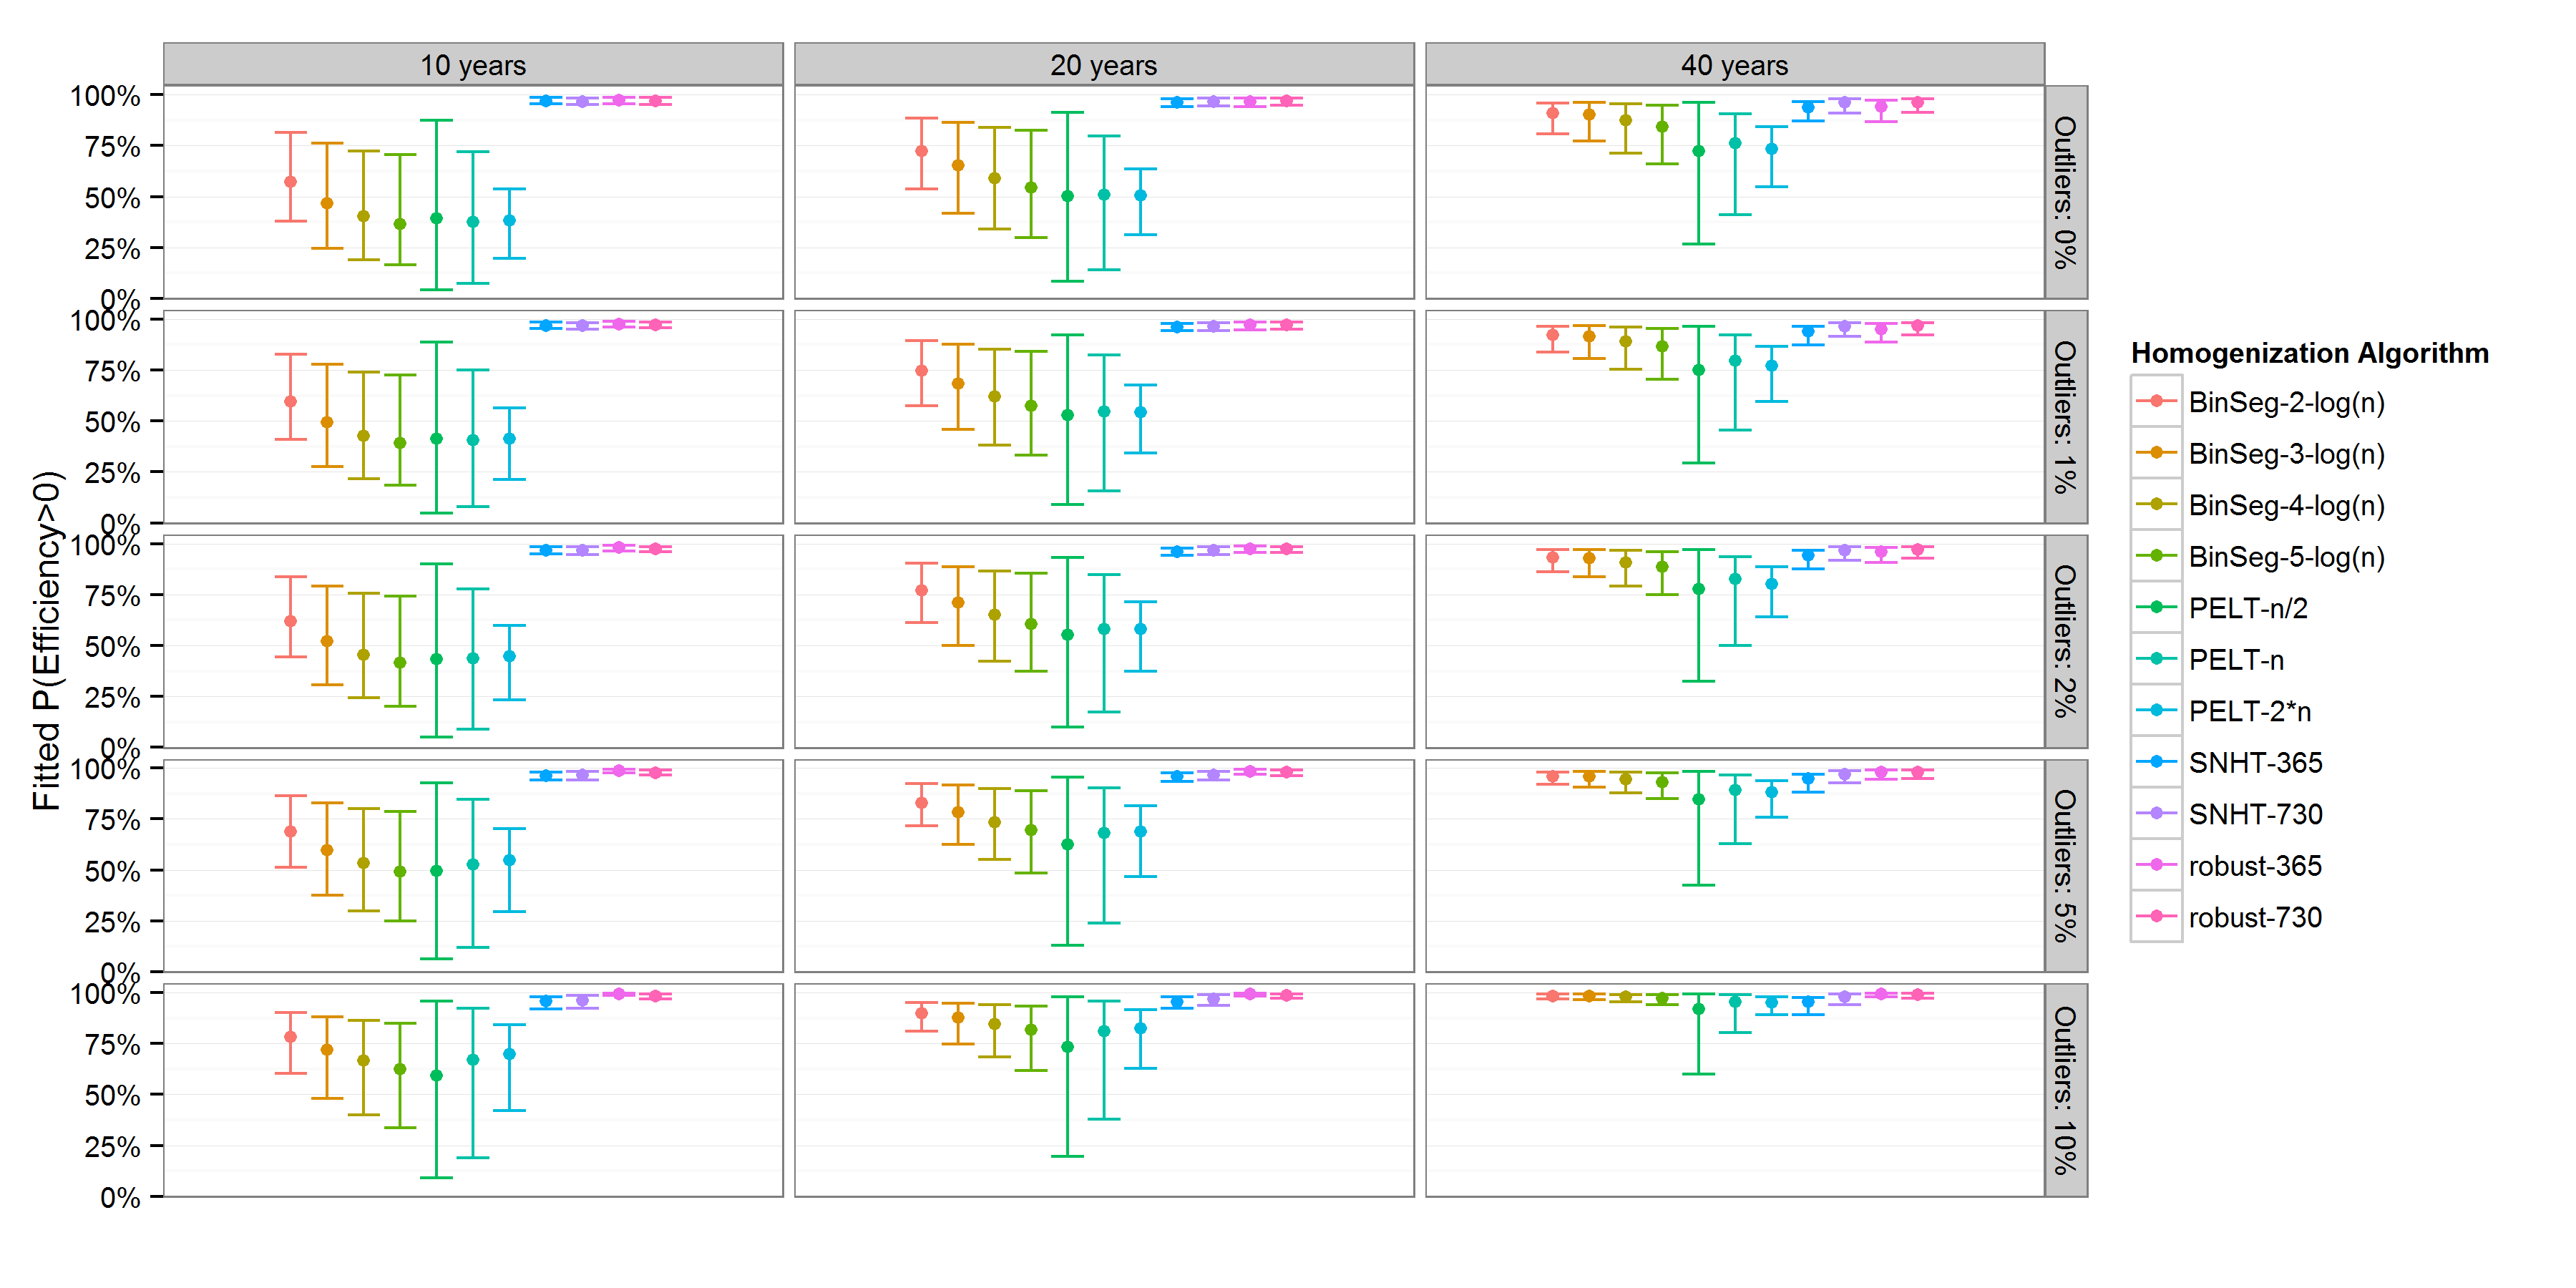
\includegraphics[width=\textwidth]{Efficiency_Model_Plot_BW}
\end{figure}
\begin{itemize}
	\item Error bars indicate the range of simulated efficiencies due to the different input time series.
	\item This graph shows the SNHT algorithms greatly outperform all other methods in most cases.
	\item A table of performance metrics is available in my thesis.
\end{itemize}
}

\frame{\frametitle{The SNHT Statistic}
\small
\begin{itemize}
	\item For each time point, the SNHT test statistic is
	\begin{equation*}
	T_i = \frac{N}{s_i}\left( (\bar{X}_{L,i}-\bar{X}_i)^2 + (\bar{X}_{R,i}-\bar{X}_i)^2\right),
	\end{equation*}
	where $\bar{X}_i$ is the mean of $\bar{X}_{L,i}$ and $\bar{X}_{R,i}$, and $s_i$ is the estimated standard deviation over the $N$ days prior and $N$ days following observation $i$.
	\item During my proposal, it was pointed out that $T_i$ will depend on the variability of the time series, and that it might be more reasonable to replace $s_i$ with $s_i^2$.
	\item In \cite{haimberger07}, the above statistic is used.  However, \cite{haimberger07} references \cite{alexandersson97} for the SNHT, and in \cite{alexandersson97} the test statistic is defined with no $s_i$ in the denominator because the $X_i$ were already standardized.
	\item Thus, $T_i$ is dependent on the variability of the time series and could be improved.  However, it should be noted that the robust SNHT outperformed all other homogenization algorithms even with this lack of standardization.
\end{itemize}
}

\frame{\frametitle{More on the SNHT Statistic}
	\small
	\vspace{-.2cm}
	\begin{figure}
		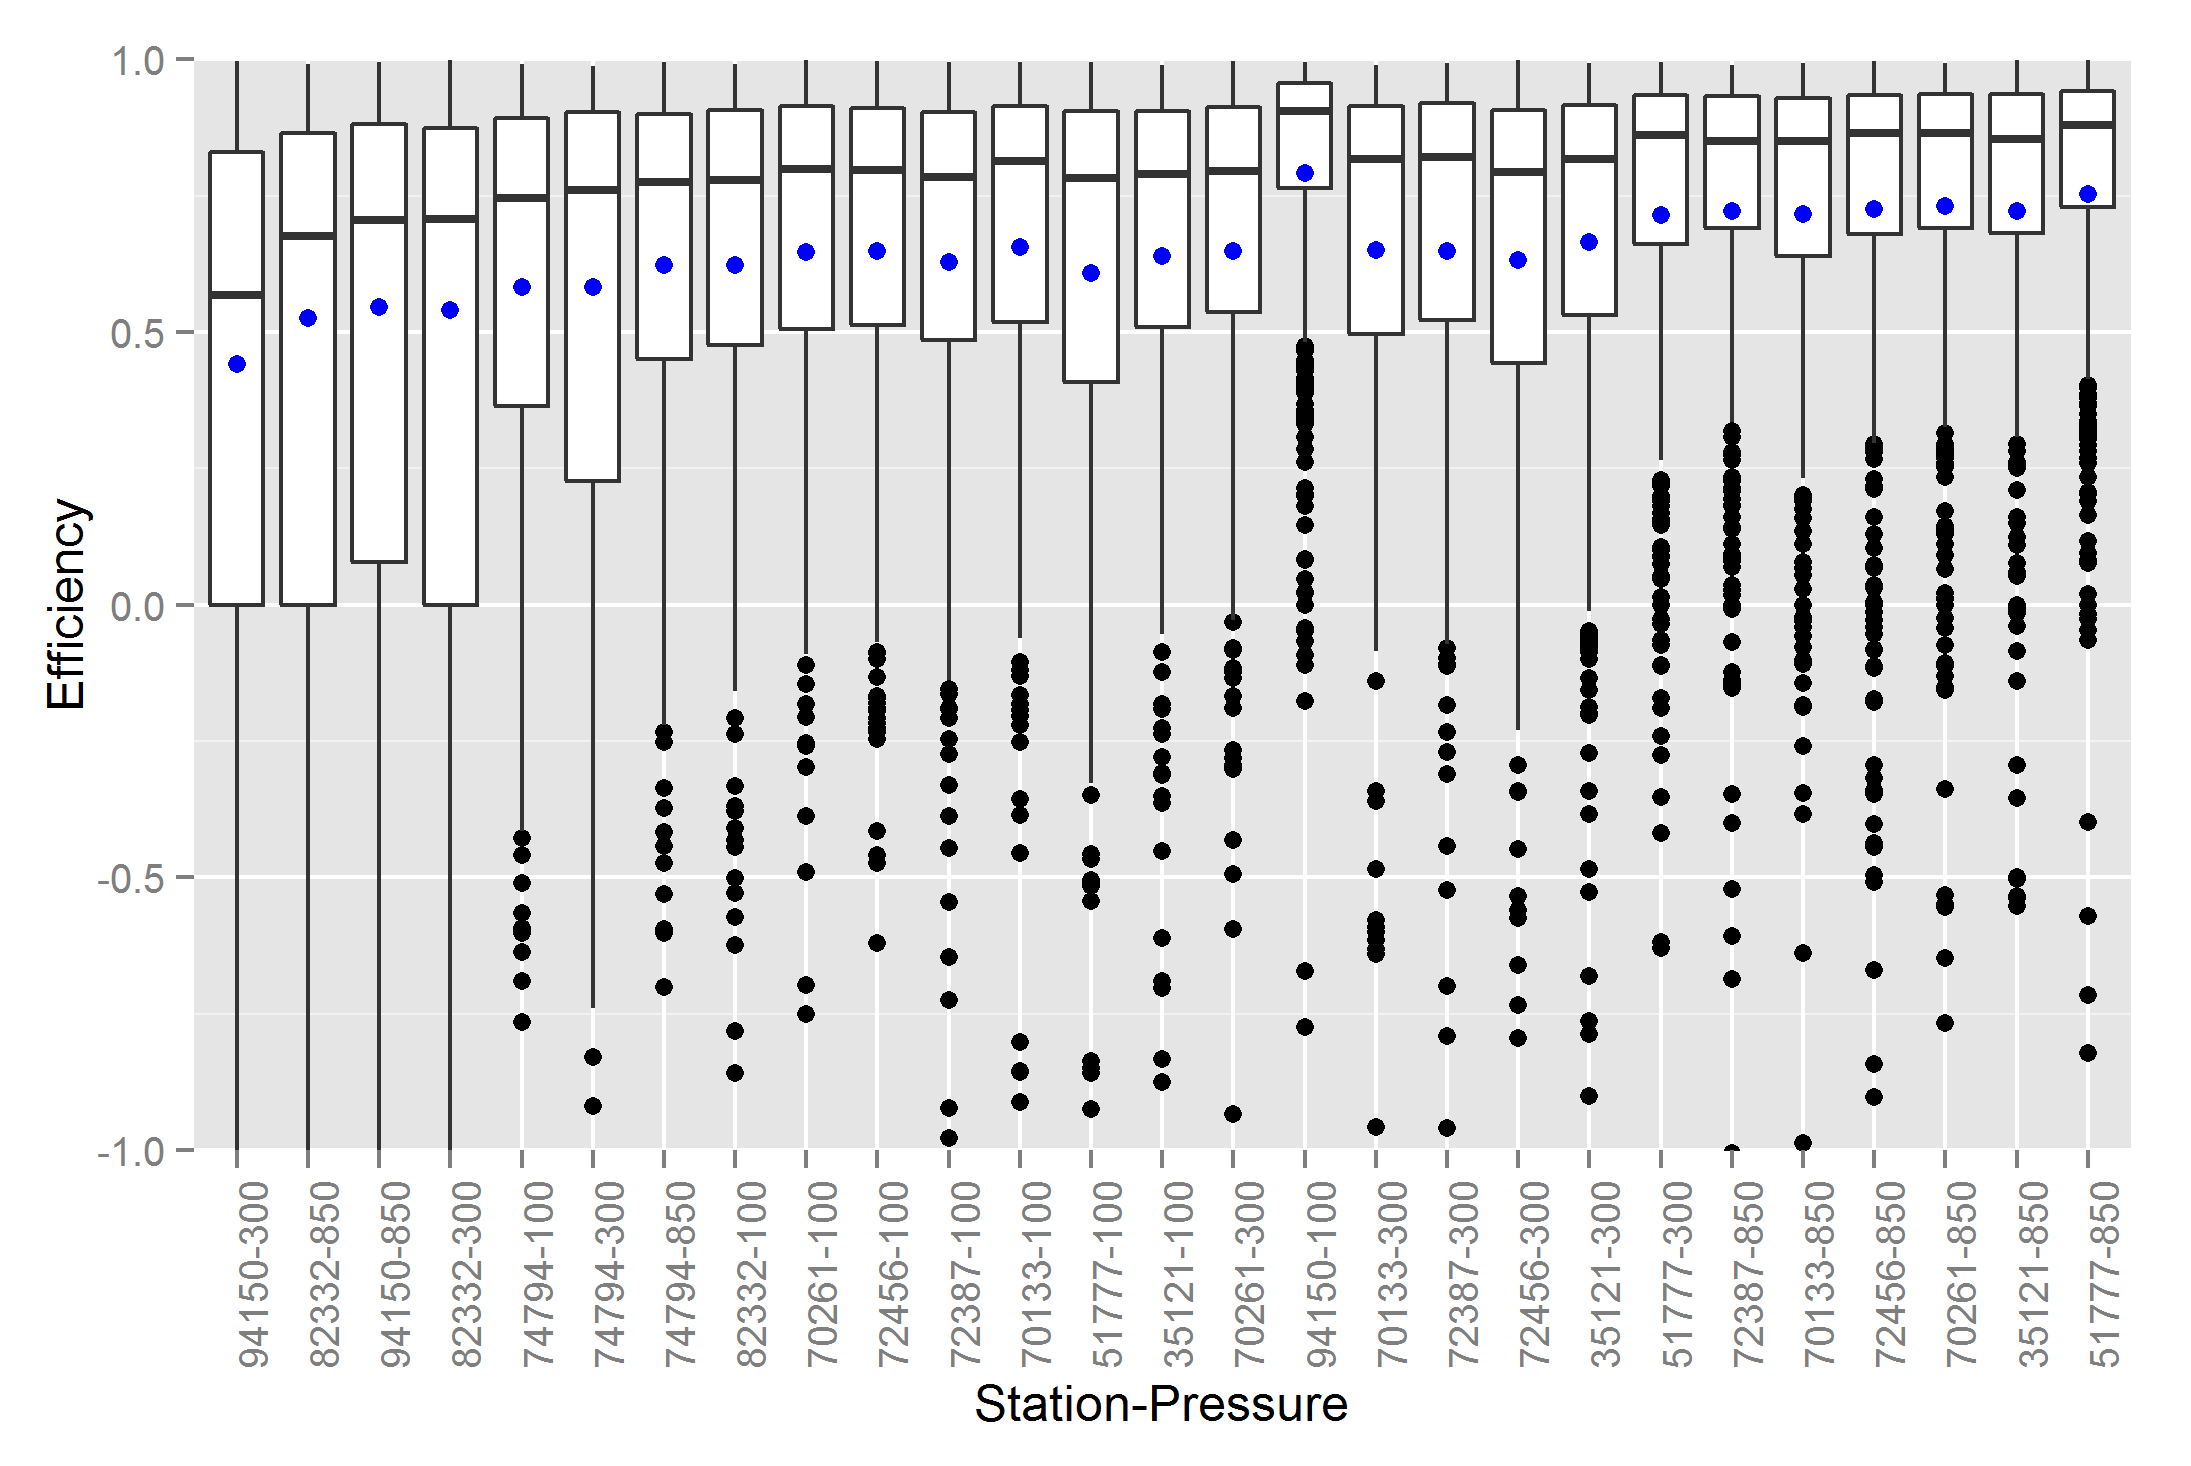
\includegraphics[width=.8\textwidth]{efficiency_by_station_robust_365}
	\end{figure}
	\vspace{-.8cm}
	\begin{itemize}
		\item The above plot has station/pressure level combinations on the $x$-axis, with the standard deviation of the station/pressure level increasing from left to right.
		\item It is clear that the efficiency is dependent on the variability of the time series, and it will also depend on the autocorrelation of the time series.
	\end{itemize}
}

\frame{\frametitle{More on the SNHT Statistic}
	\begin{itemize}
		\item I plan on fixing this issue by replacing the original SNHT statistic with the correct statistic:
		\begin{align*}
			T_i &= \frac{N}{s_i^2}\left( (\bar{X}_{L,i}-\bar{X}_i)^2 + (\bar{X}_{R,i}-\bar{X}_i)^2\right)\\
			&= \frac{2N}{s_i^2} (\bar{X}_{L,i}-\bar{X}_{R,i})^2
		\end{align*}
		\item Additionally, $s_i$ will account for the autocorrelation of the time series $\mathbf{X}$, and thus $T_i$ will be proportional to a $\chi^2_1$ (provided $\mathbf{X}$ is stationary and normal with a varying mean).
	\end{itemize}
}

\subsection{Sequencings}

\frame{\frametitle{Logistic Model Deviances}
\begin{table}[ht]
	\tiny
	\centering
	\begin{tabular}{l|cc|cc|cc}
		\hline
		& \multicolumn{2}{c|}{\textbf{TPR}} & \multicolumn{2}{c|}{\textbf{FPR}} & \multicolumn{2}{c}{\textbf{Efficiency}}\\
		Model Type & Deviance & \% Reduction & Deviance & \% Reduction & Deviance & \% Reduction\\
		\hline
		Intercept Only & 6240630 & --- & 5835529 & --- & 159942 & ---\\
		Main Effects  & 4631181 & 25.79\% & 1244423 & 78.68\% & 136467 & 14.68\%\\
		2-Way Interactions  & 4101383 & 11.44\% & 279232 & 77.56\% & 132980 & 2.56\%\\
		3-Way Interactions  & 4058965 & 1.03\% & 258216 & 7.53\% & 132585 & 0.30\%\\
		4-Way Interactions  & 4049724 & 0.23\% & 255145 & 1.19\% & 132421 & 0.12\%\\
		5-Way Interactions  & 4047592 & 0.05\% & 254845 & 0.12\% & 132411 & 0.01\%\\
		\hline
	\end{tabular}
\end{table}
\begin{itemize}
	\item Similar to the homogenization algorithm comparison, I fit a logistic regression model to the true positive, false positive, and efficiency results for the sequencing study.
	\item In all cases, I chose to use the 2-way interaction model, as that model seemed to attain a good deviance without too much complexity.
\end{itemize}
}

\frame{\frametitle{True Positive Rate Results}
\begin{figure}
	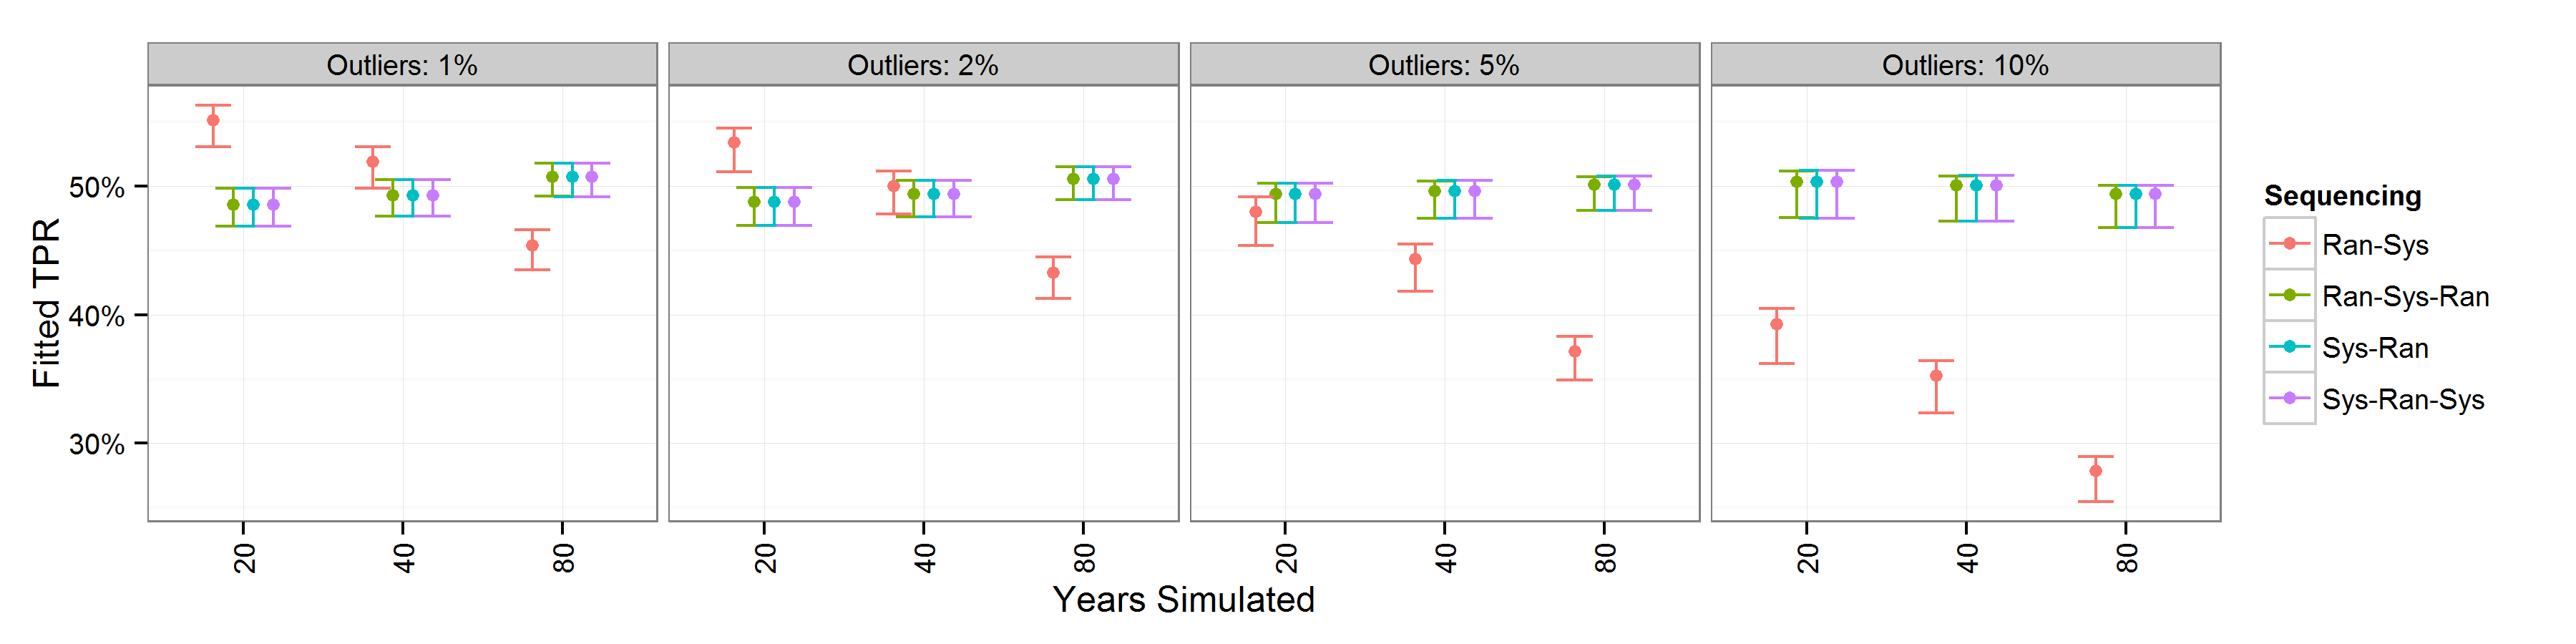
\includegraphics[width=\textwidth]{TPR_Order_Plot}
\end{figure}
\begin{itemize}
	\item In most cases, the true positive rate is maximized with a sequencing that has a random error check following a systematic error correction.
	\item The few exceptions are with small datasets and small contamination rates.
	\item There are very few differences between the other 3 sequencings considered.
\end{itemize}
}

\frame{\frametitle{False Positive Rate Results}
\begin{figure}
	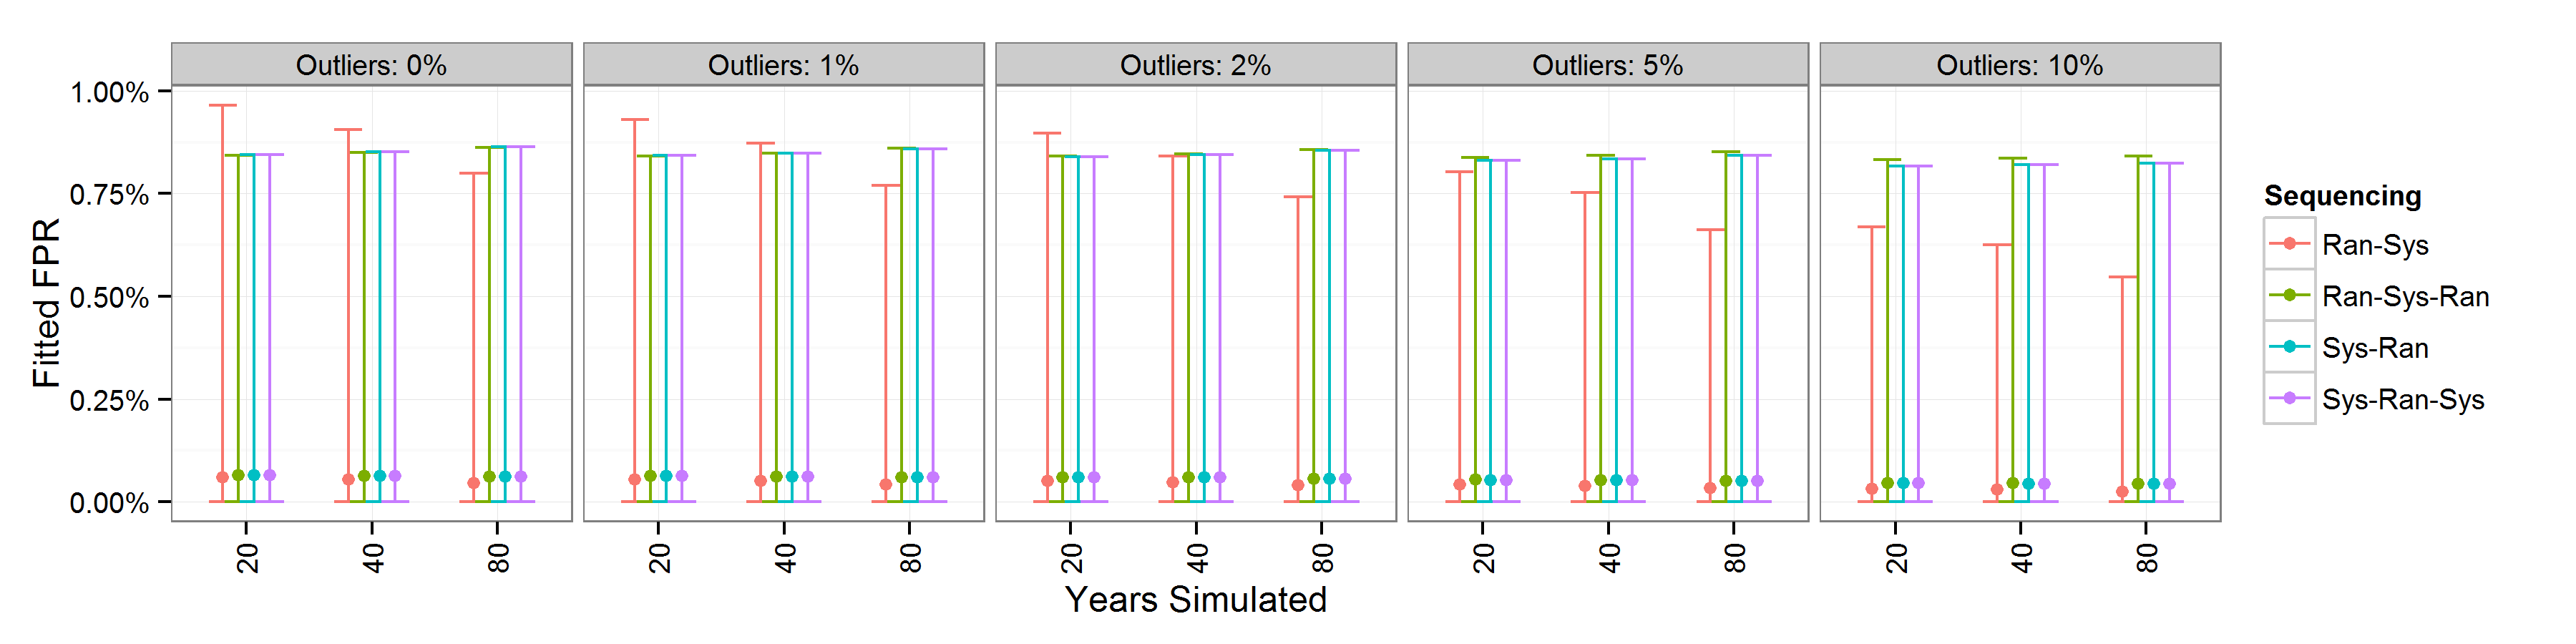
\includegraphics[width=\textwidth]{FPR_Order_Plot}
\end{figure}
\begin{itemize}
	\item I again see more variability in the ``Ran-Sys'' sequencing.
	\item All false positive rates are extremely low, and I see no reason for choosing one sequencing over another based on these False Positive Rate alone.
\end{itemize}
}

\frame{\frametitle{Efficiency Results}
\begin{figure}
	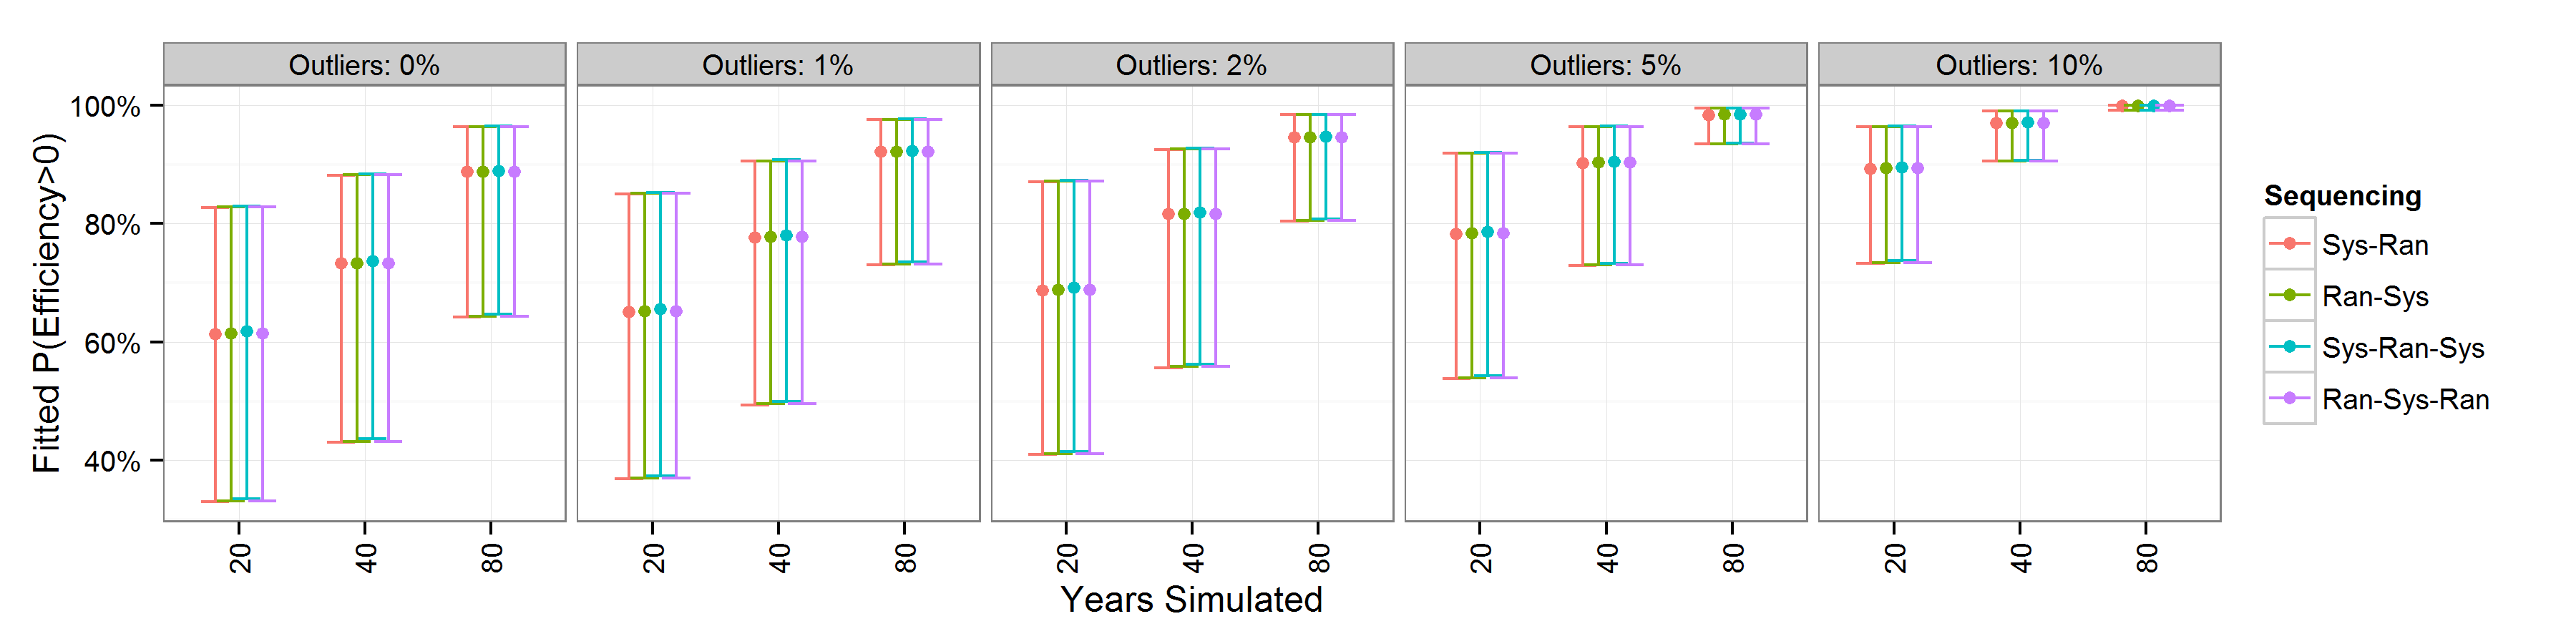
\includegraphics[width=\textwidth]{Efficiency_Order_Plot}
\end{figure}
\begin{itemize}
	\item Again, there are very little differences between the four proposed sequencings.
\end{itemize}
}

\subsection{Conclusion}

\frame{\frametitle{Conclusion}
\begin{itemize}
	\item The Robust SNHT achieves the highest efficiency across all homogenization algorithms.
	\item I recommend the sequence ``Sys-Ran'' for quality controlling radiosonde data.  It outperforms ``Ran-Sys'' at detecting true errors, and is comparable in all other cases.
	\item I do not recommend the sequencings ``Sys-Ran-Sys'' or ``Ran-Sys-Ran'' as they do not appear to show any improvement over ``Sys-Ran'' and are certainly more computationally expensive.
\end{itemize}
}


\section{Case Study}

\frame{\frametitle{Station 70219- Bethel, Alaska, USA}
\begin{figure}
	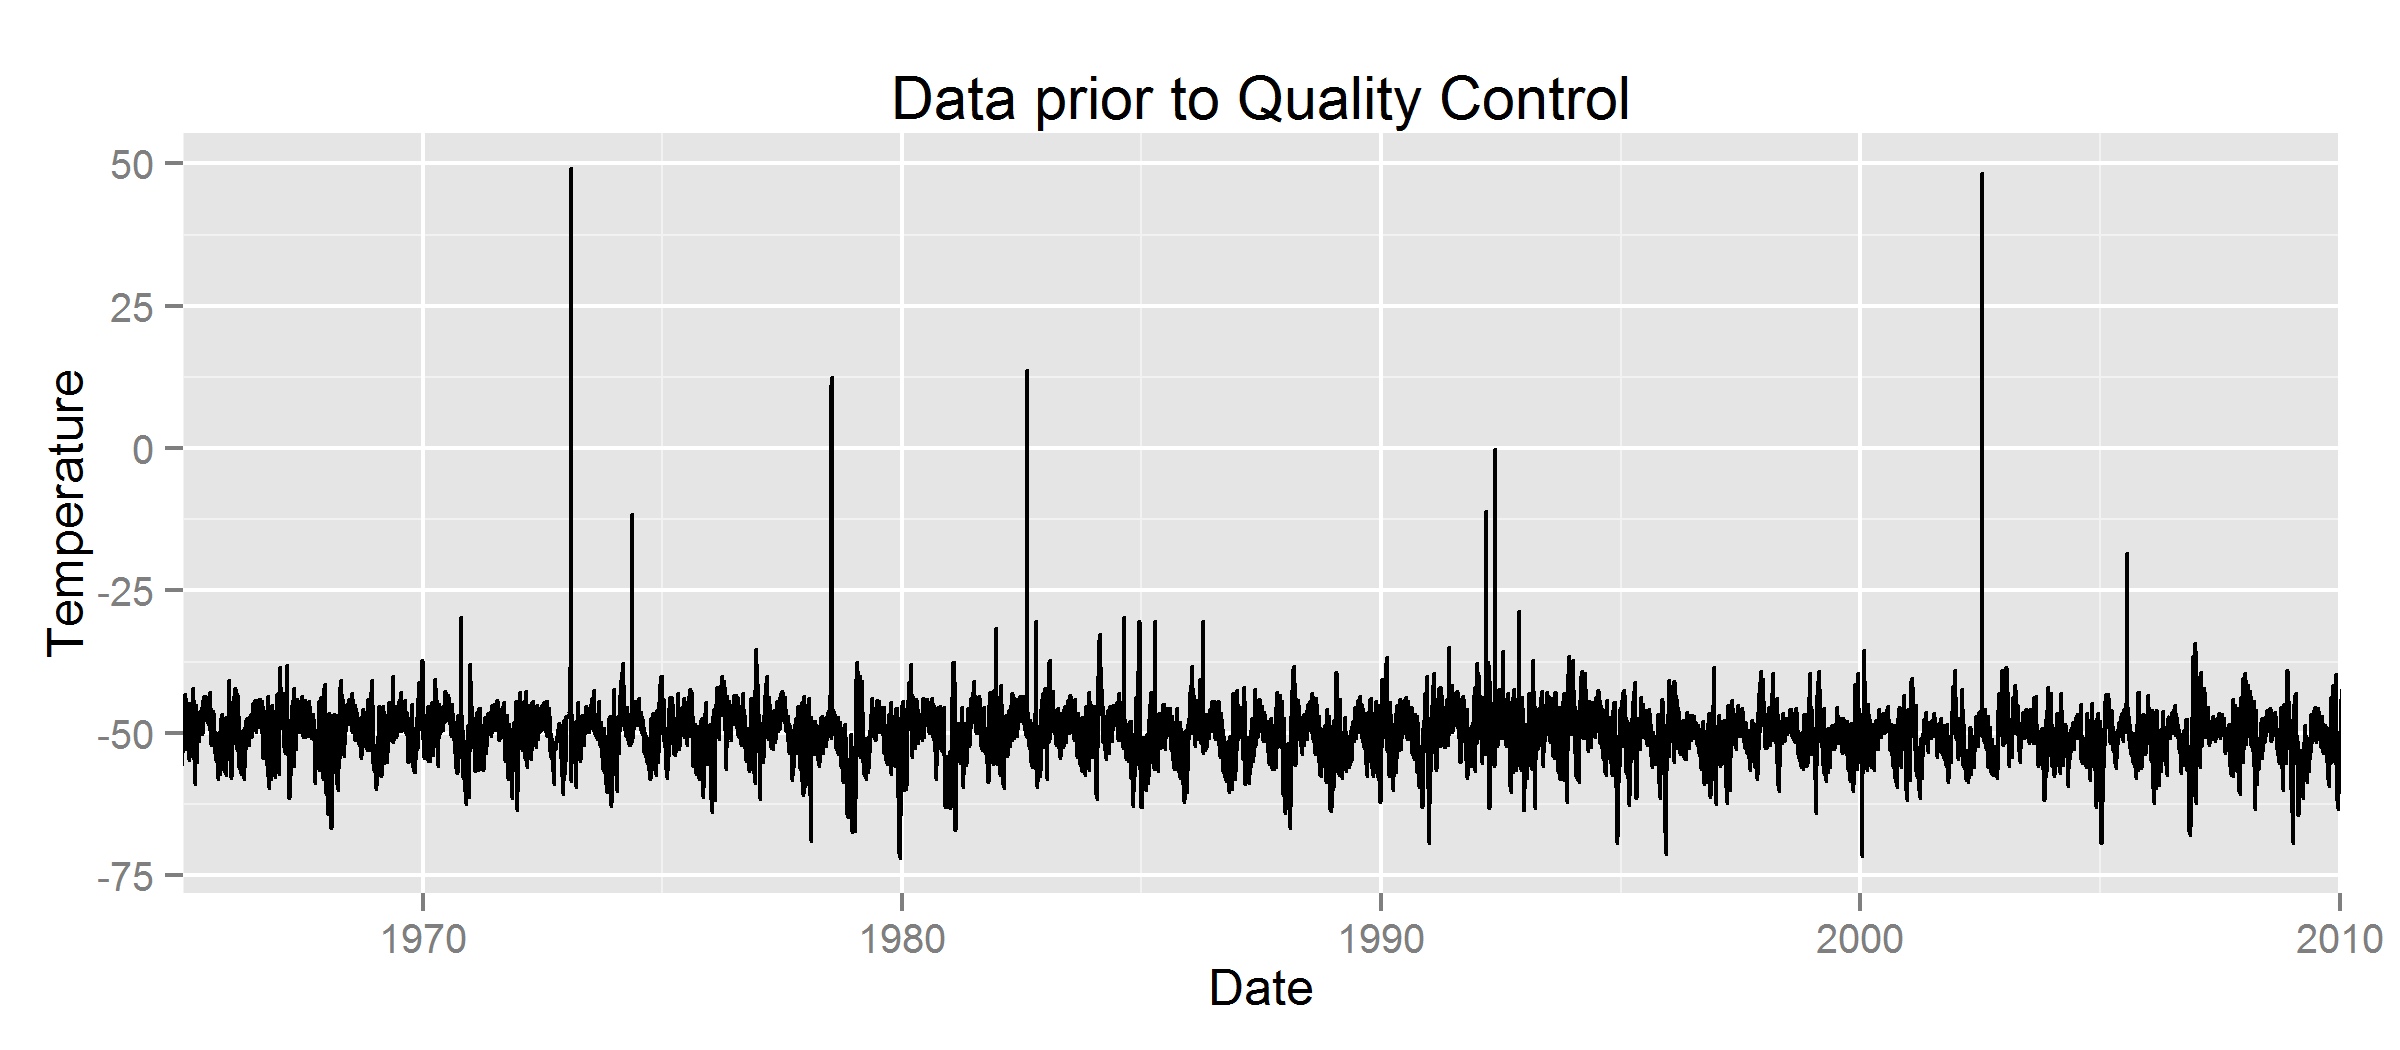
\includegraphics[width=\textwidth]{70219_Data_Unhomogenized_no_vlines}
\end{figure}
\begin{itemize}
	\item This plot shows several obvious random errors in a radiosonde temperature dataset.
	\item Systematic errors are harder to detect my eye, especially at this scale.
\end{itemize}
}

\frame{\frametitle{Random Errors Removed}
\begin{figure}
	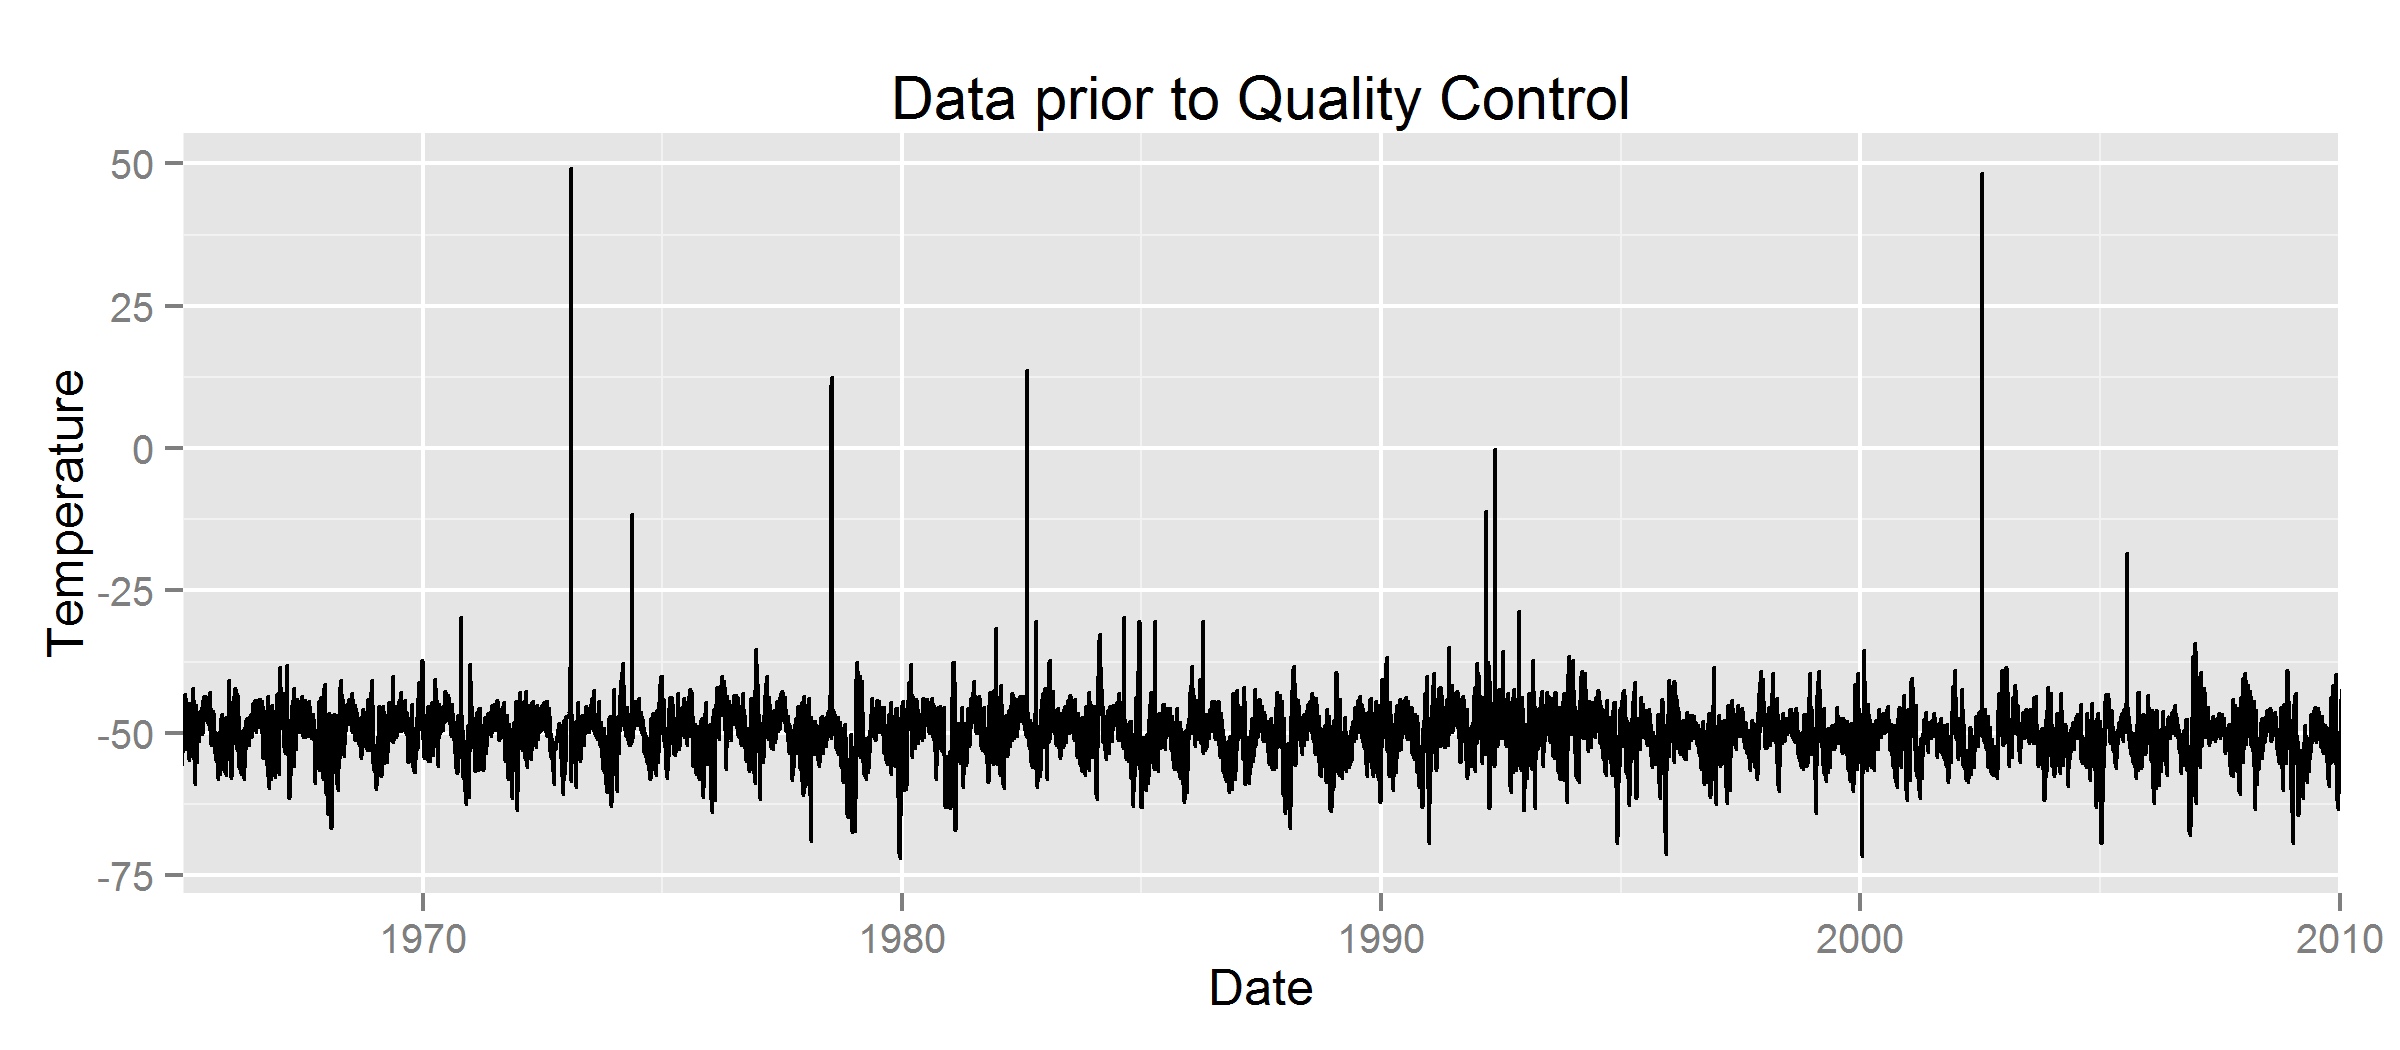
\includegraphics[width=.9\textwidth]{70219_Data_Unhomogenized_no_vlines}\\
	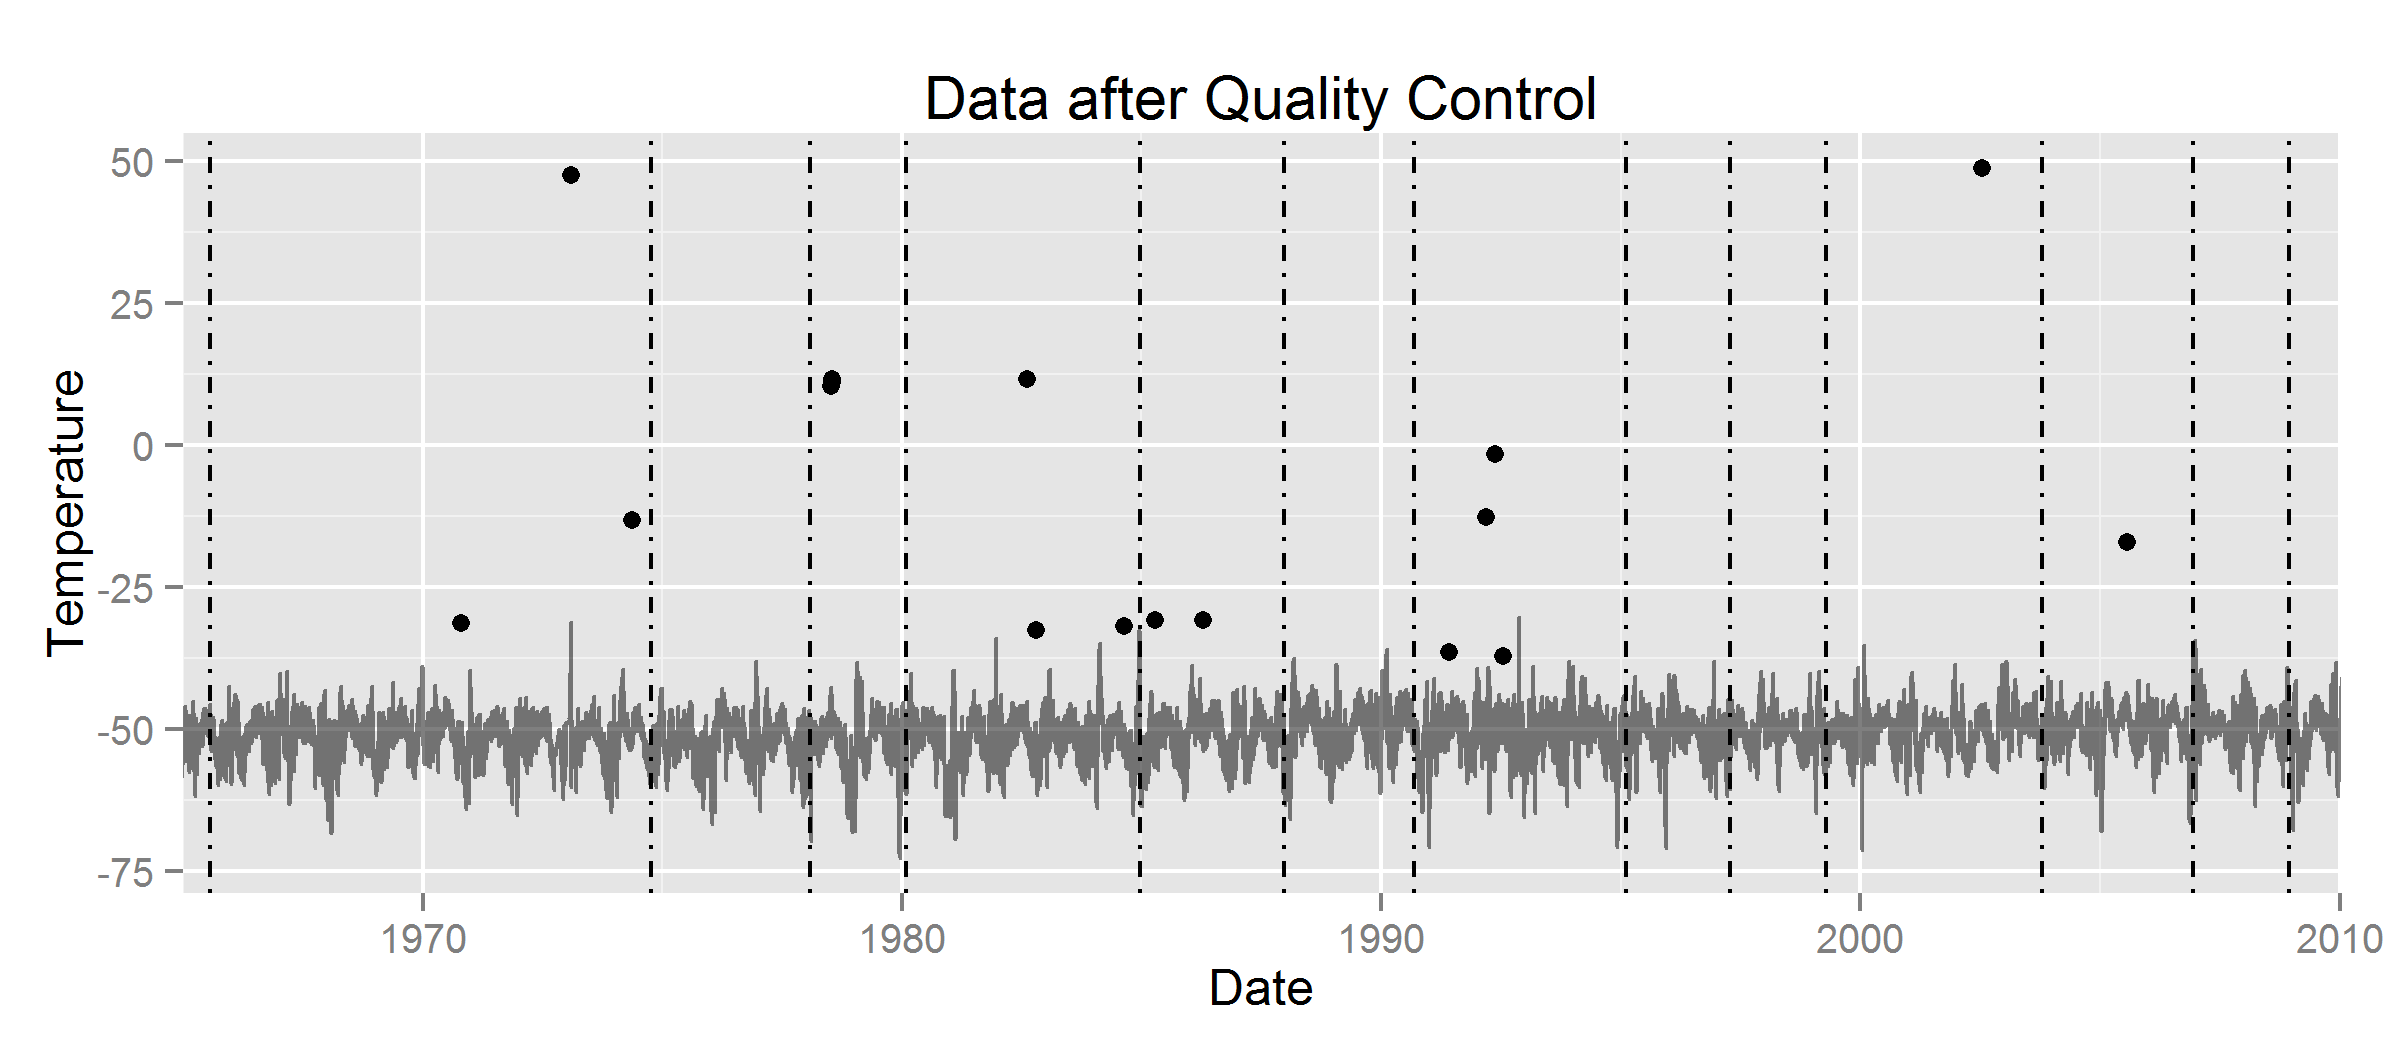
\includegraphics[width=.9\textwidth]{70219_Data_Homogenized}
\end{figure}
}

\frame{\frametitle{Systematic Errors Corrected}
	\begin{figure}
		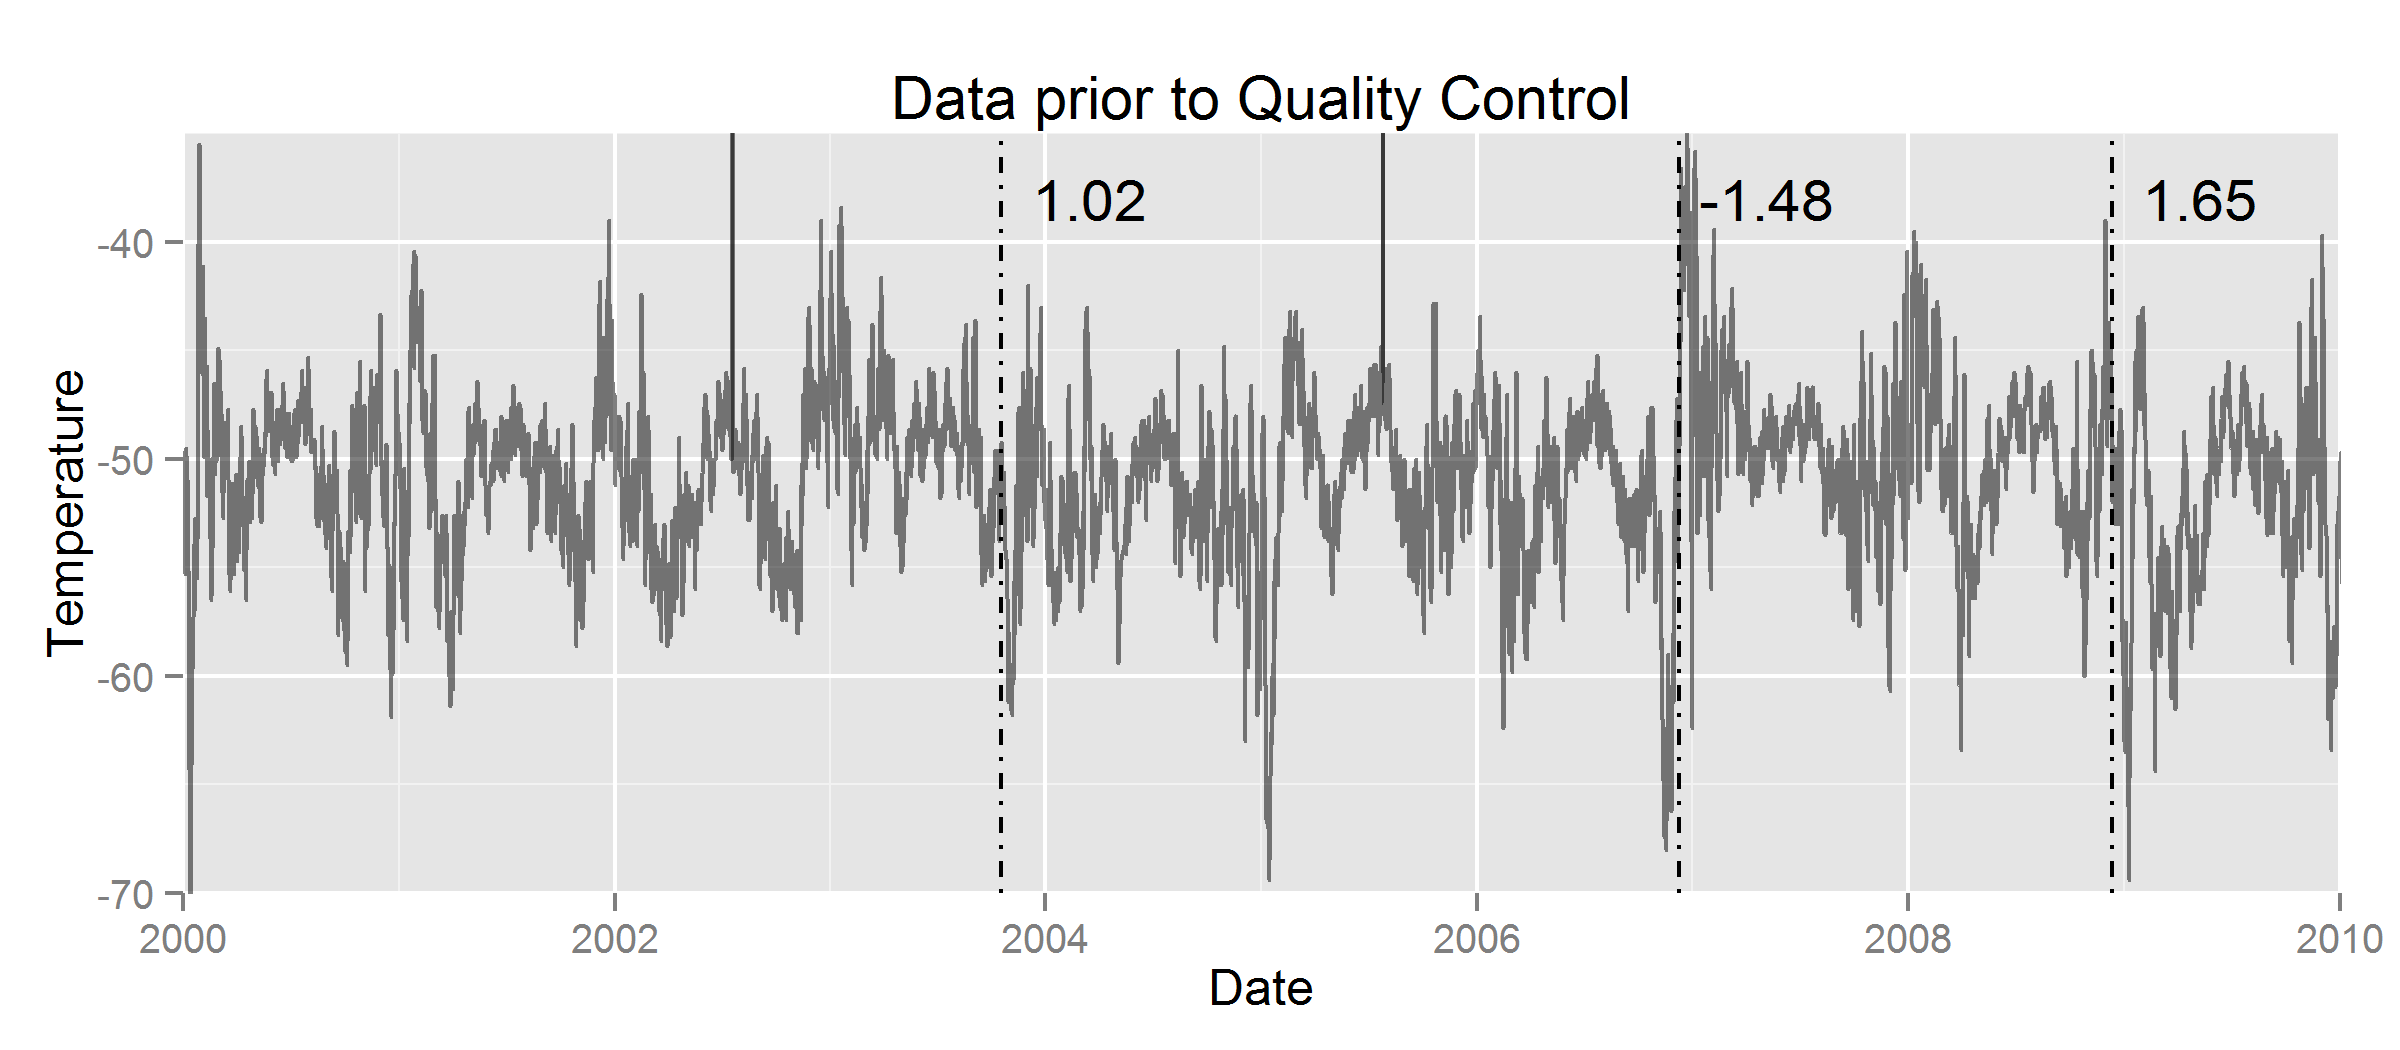
\includegraphics[width=.9\textwidth]{70219_Data_Unhomogenized_zoomed}\\
		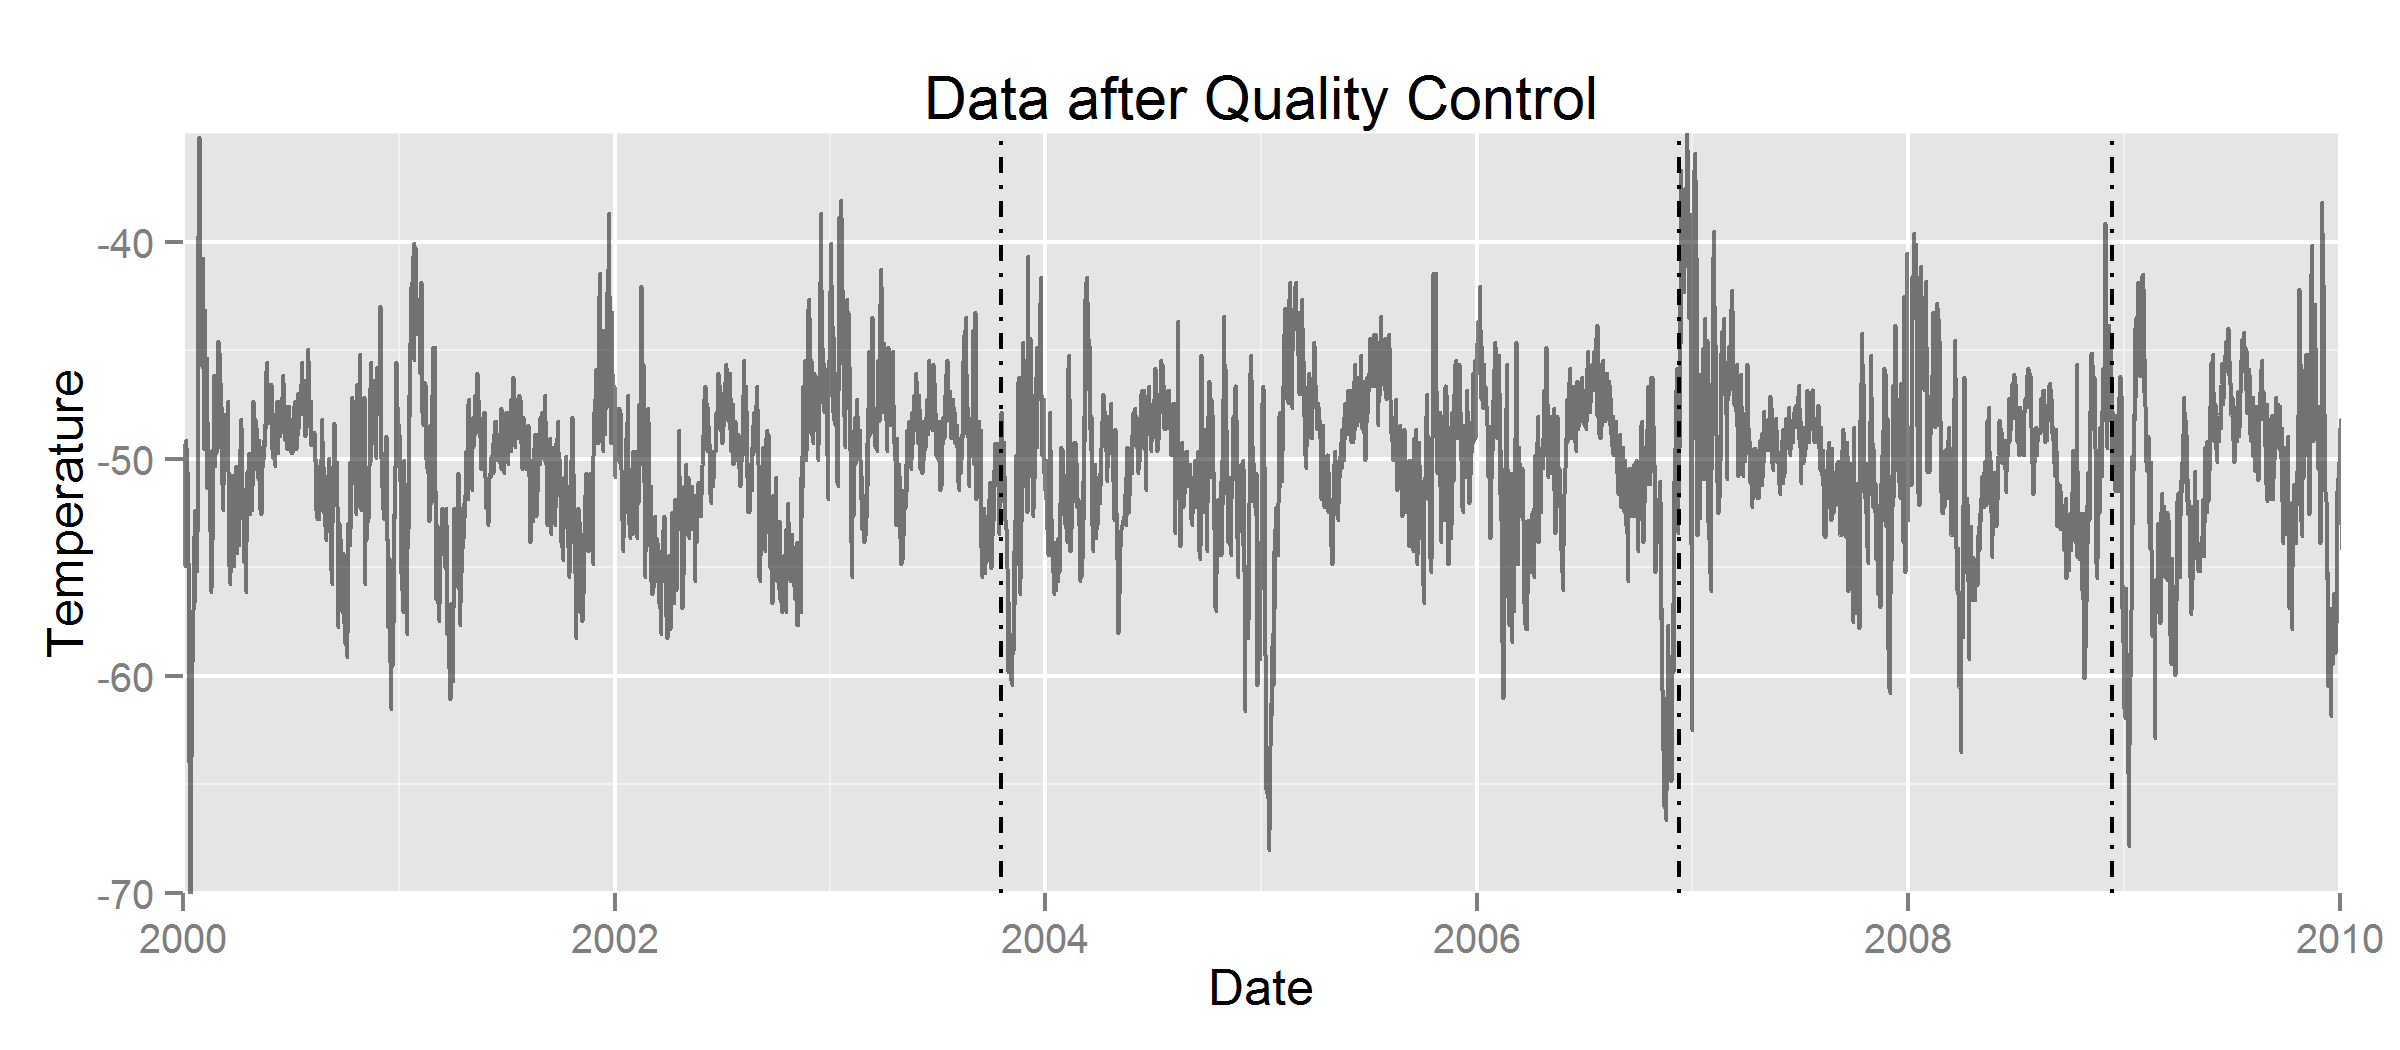
\includegraphics[width=.9\textwidth]{70219_Data_Homogenized_zoomed}
	\end{figure}
}

\frame{\frametitle{Future Work}
	\begin{itemize}
		\item Redefine the SNHT statistic to
		\begin{itemize}
			\item Correctly standardize by $s^2$ instead of $s$.
			\item Robustly estimate the variance.
			\item Model the temporal dependence and the influence this has on the variability of the sample means.
		\end{itemize}
		\item Determine the sampling distribution of the test statistic in order to determine a threshold for systematic error detection.
		\item Apply the Benjamini-Hochberg correction for multiple dependent tests in order to appropriately adjust the threshold.
	\end{itemize}
}
	
\section{References}

\frame[shrink=30]{\frametitle{References}
	\footnotesize
	\bibliographystyle{myabbrvnat}
	\bibliography{mybib}
}

\section{Appendix}

\part{2}

\frame{\frametitle{Appendix}\tableofcontents[currentsection]} 

\section{Radiosonde Data}

\frame{\frametitle{Radiosonde Data}
	\begin{columns}
		\begin{column}{.3\textwidth}
			\begin{figure}
				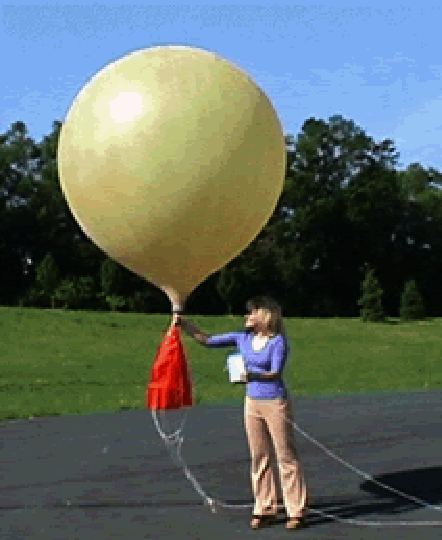
\includegraphics[width=.7\textwidth]{radiosonde_launch-eps-converted-to.pdf}
				\caption{Sample Radiosonde}
				\label{fig:radio}
			\end{figure}
			\begin{figure}
				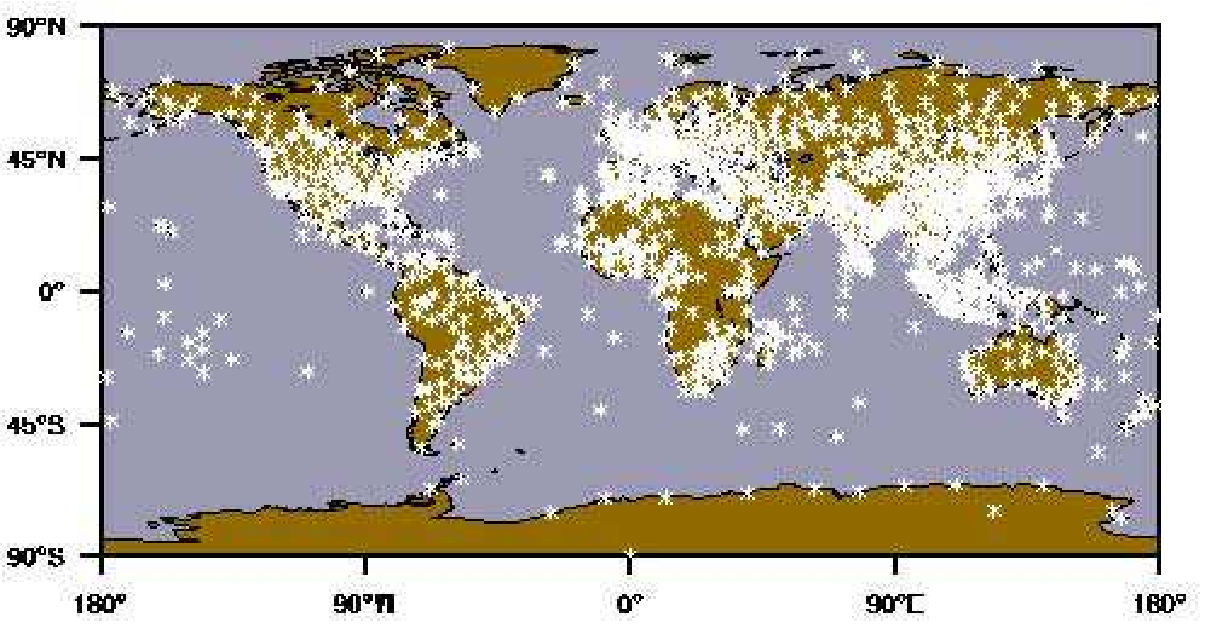
\includegraphics[width=\textwidth]{GlobalRadiosondeNetwork2-eps-converted-to.pdf}
				\caption{Global Radiosonde Network}
				\label{fig:global}
			\end{figure}
		\end{column}
		\begin{column}{.7\textwidth}
			\begin{itemize}
				\item Small instruments are suspended below 2m hydrogen or helium balloons.
				\item They measure atmospheric variables such as temperature, wind speed, etc.
				\item Balloons are launched twice daily at roughly 00 UTC and 12 UTC, and at 700 sites worldwide.
				\item More than 1,300 additional launch sites exist in the historical archive.
				\item Considering the number of launch sites, multiple observations for different pressure levels, and the total number of launches, there are between 50 and 90 million historical soundings.
			\end{itemize}
		\end{column}
	\end{columns}
}

\section{Robust Mean and Standard Deviation}

\frame{\frametitle{Robust Mean and Standard Deviation}
	\footnotesize
	\begin{enumerate}
		\item First, the estimates of the mean, $\hat{\mu}$, and standard deviation, $\hat{\sigma}$, are initialized to
		\begin{align*}
		\hat{\mu} &= \mbox{median}(\mathbf{x})\\
		\hat{\sigma} &= \mbox{MAD}(\mathbf{x}),
		\end{align*}
		where $\mathbf{x}$ is a vector of the data, and $MAD$ is the median absolute deviation, defined as
		\begin{equation*}
		MAD = \mbox{median}( \lvert x_i - \mbox{median}(\mathbf{x}) \rvert ).
		\end{equation*}
		\item Then, Winsorized values, $y_i$, are computed.  These are defined as
		\begin{equation*}
		y_i = \left\{ \begin{array}{ll}
		\hat{\mu}-k \hat{\sigma} & : x_i \leq \hat{\mu}-k \hat{\sigma}\\
		x_i & : \hat{\mu}-k \hat{\sigma} < x_i \leq \hat{\mu}+k \hat{\sigma}\\
		\hat{\mu}+k \hat{\sigma} & : x_i > \hat{\mu}+k \hat{\sigma}\\
		\end{array} \right.
		\end{equation*}
		\item Updated estimates of $\hat{\mu}$ and $\hat{\sigma}$ are computed as the mean of $\mathbf{y}$ and the standard deviation of $\mathbf{y}$, respectively.
		\item Steps 2 and 3 are repeated until $\hat{\mu}$ changes by less than $10^{-6} \hat{\sigma}$.
	\end{enumerate} 
	Note: In step 3, one may choose to estimate $\hat{\sigma}_L$ and $\hat{\sigma}_R$ using only observations to the left and right, respectively, of the mean.  This allows for improved outlier detection with skewed data.
}

\section{Homogenization Methods}

\frame{\frametitle{Homogenization Methods: SNHT}
	\small
	This algorithm is commonly used in the climate literature.  The algorithm works as follows:
	\begin{enumerate}
		\item For each observation, two means are computed: one for the $N$ days prior to observation $i$, $\bar{X}_{L,i}$, and one for the $N$ days following, $\bar{X}_{R,i}$
		\item Then, the test statistic
			\begin{equation}
			T_i = \frac{N}{s_i}\left( (\bar{X}_{L,i}-\bar{X}_i)^2 + (\bar{X}_{R,i}-\bar{X}_i)^2\right),
			\label{eq:Hom}
			\end{equation}
		is computed where $\bar{X}_i$ is the mean of $\bar{X}_{L,i}$ and $\bar{X}_{R,i}$, and $s_i$ is the estimated standard deviation over the $N$ days prior and $N$ days following observation $i$.  \item If the largest $T_i$ exceeds some threshold at time $i=i^*$, I conclude that a change point occurred at time $i^*$, and I adjust all observations after time $i^*$ by $\bar{X}_{L,i^*}-\bar{X}_{R,i^*}$.  A threshold of 100 is recommended in \cite{haimberger07}.
		\item Repeat steps 1-3 until no test statistic exceeds the threshold.
	\end{enumerate}
}

\frame{\frametitle{Homogenization Methods: Robust SNHT}
	\begin{itemize}
		\item The previous algorithm is not robust to random errors, as the influence function for the sample mean is unbounded.
		\item The Winsorized estimator of center and scale discussed previously is robust against random errors.
		\item Thus, to create a robust SNHT statistic, I propose replacing the means and standard deviation in Equation~(\ref{eq:Hom}) with these estimators.
	\end{itemize}
}

\frame{\frametitle{Homogenization Methods: BinSeg}
	\begin{itemize}
		\item Several homogenization methods work by optimizing a cost function:
		\begin{equation}
		\sum_{i=1}^{m+1} [\mathcal{C}(y_{(\tau_{i-1}+1):\tau_i})] + \beta f(m),
		\label{eq:cost}
		\end{equation}
		where $\tau_i$ is the $i$th change point; $m$ is the number of change points; $\mathcal{C}$ is a cost function; $y_{(\tau_{i-1}+1):\tau_i}$ is the observed data between the $(i-1)$ and $i$th change point; and $\beta f(m)$ is a penalty term on the number of change points, see \cite{killick12}.
		\item Often, $\mathcal{C}$ is chosen to be twice the negative log likelihood, and $f(\cdot)$ is linear.
		\item Binary Segmentation (BinSeg) uses a greedy algorithm: at each step, a changepoint is selected which minimizes the cost function.  The data is then partitioned in two, and optimization continues iteratively.
	\end{itemize}
}

\frame{\frametitle{Homogenization Methods: PELT}
	\begin{itemize}
		\item Pruned Exact Linear Time (PELT) is another algorithm for optimizing Equation (\ref{eq:cost}), but it computes the exact minimum.
		\item It proceeds recursively as follows: first, the optimal number and location of change points is determined for observations 1 and 2 only.  The optimal number and location of change points for the first three observations is then determined using this information, and more generally the optimal number and location of change points for the first $k+1$ observations is determined by considering the optimal configurations for the first $2, 3, \ldots, k$ observations.
		\item PELT is computationally efficient, and is implemented in the \texttt{changepoint} package in R \cite{killick14}.
	\end{itemize}
}

\section{Modeling Radiosonde Data}

\frame{\frametitle{Modeling Radiosonde Data- Part 1}
	\begin{enumerate}
		\item In order to capture seasonal and hourly trends, I plan on fitting a Generalized Additive Model (GAM) to the radiosonde temperature data.
		\item GAMs are flexible, non-parametric models that allow the response variable to be a linear combination of smoothed functions of the input variables, see \cite{hastie90}.
		\item The particular model I'll fit is
		\begin{equation} \label{eq:GAM}
		t_i = \beta_0 + s_1(h_i) + s_2(d_i) + \beta_1 y_i + \epsilon_i,
		\end{equation}
		where $t_i$ is the temperature at a given station and pressure level; $h_i$, $d_i$ and $y_i$ are the hour, day, and year of the $i$-th observation, respectively; $\beta_0$ is the intercept; $\beta_1$ is the coefficient for the long term trend; and $s_1(\cdot)$ and $s_2(\cdot)$ are cubic regression splines.
	\end{enumerate}  
}

\frame{\frametitle{Modeling Radiosonde Data- Part 2}
	\begin{enumerate}
		\item Typically the error term, $\epsilon_i$, in the GAM model would be modeled as normal with some unknown variance, but the distribution of the error terms could be skewed or have heavier tails than a normal distribution.
		\item Thus, I'll use a skew-$t$ distribution for the errors of this model, which has 4 parameters, $\xi, \sigma, \alpha$, and $\nu$ which are useful in controlling the first four moments of the distribution, see \cite{azzalini03}.
	\end{enumerate}
}

\frame{\frametitle{Modeling Radiosonde Data- Part 3}
	\begin{enumerate}
		\small
		\item Additionally, I expect there to be temporal correlation in the error terms.
		\item Since I have already included hourly and seasonal terms in the model, I expect most of this autocorrelation to be explained, and so an AR(1) time series model is sufficient to account for the remaining structure in the residuals.
		\item For radiosonde data, observations are not equally spaced in time:  Launches are scheduled globally at 0 and 12 UTC, but many deviations from this pattern are observed.
		\item Thus, to estimate the lag-$h$  autocorrelation, ${\phi}(h)$, in hours, I must use only those observations that are $h$ time steps apart:
		\begin{equation} \label{eq:ACF}
		\widehat{\phi}(h)=\frac{1}{\lvert \mathcal{P}_h\rvert} \sum_{(\widehat{\epsilon_i},\widehat{\epsilon_j}) \in \mathcal{P}_h} \frac{(\widehat{\epsilon_i}-\bar{\epsilon_i})(\widehat{\epsilon_j}-\bar{\epsilon_j})}{\sqrt{s_{\epsilon_i} s_{\epsilon_j}}},
		\end{equation}
		where $\mathcal{P}_h$ is the set of all pairs of residuals that are $h$ hours apart (or within some window), and $\widehat{\epsilon_i}$ is the observed residual from Equation~(\ref{eq:GAM}).
		\item For an AR(1) model, I need only estimate $\phi(\cdot)$ at $h=12$ hours, and I plan on using a window of 5\% of 12 hours, or 0.6 hours.
	\end{enumerate}
}

\frame{\frametitle{Modeling Radiosonde Data- Part 4}
	\begin{enumerate}
		\item After a simulated dataset is generated, it is contaminated with random and systematic errors.
		\item Random errors are generated by sampling 1, 2, 5 or 10\% of the observations and adding or subtracting a random error following a distribution of $N(10\sigma, 1\sigma^2)$, where $\sigma^2$ is the standard deviation of the simulated series, estimated from the GAM model.
		\item Systematic errors are generated by sampling 1, 2, or 3 observations uniformly per simulated decade and then drawing a break size from a $N(0, 0.04\sigma^2)$. The break size is then added to all observations after the change point.
	\end{enumerate}
}

\section{Variance of the SNHT Statistic}

\frame{\frametitle{Variance of the SNHT Statistic}
	\begin{itemize}
		\item The new test statistic is
		$$T_i = \frac{2N}{s_i^2} (\bar{X}_{L,i}-\bar{X}_{R,i})^2$$
		where $s_i^2$ is the variance of $\bar{X}_{Li}-\bar{X}_{Ri}$.
		\item I will assume the $X_i$ are normal with some mean that depends on the hour of the day and the day of the year.
		\item $\bar{X}_{Li}-\bar{X}_{Ri}$ will then be normal with mean 0 (assuming $\mathbf{X}$ is stationary) with variance
		$$\frac{1}{N^2} (\mathbf{1}, -\mathbf{1}) \Sigma (\mathbf{1}, -\mathbf{1})^T$$
		where $\mathbf{1}$ is a vector of $N$ 1's and $\Sigma$ is the $2N \times 2N$ covariance matrix for $X_{i-N}, X_{i-N+1}, \ldots, X_{i-2}, X_{i-1}, X_{i+1}, X_{i+2}, \ldots, X_{i+N}$.
	\end{itemize}
}

\frame{\frametitle{Modeling $\Sigma$}
	\begin{figure}
		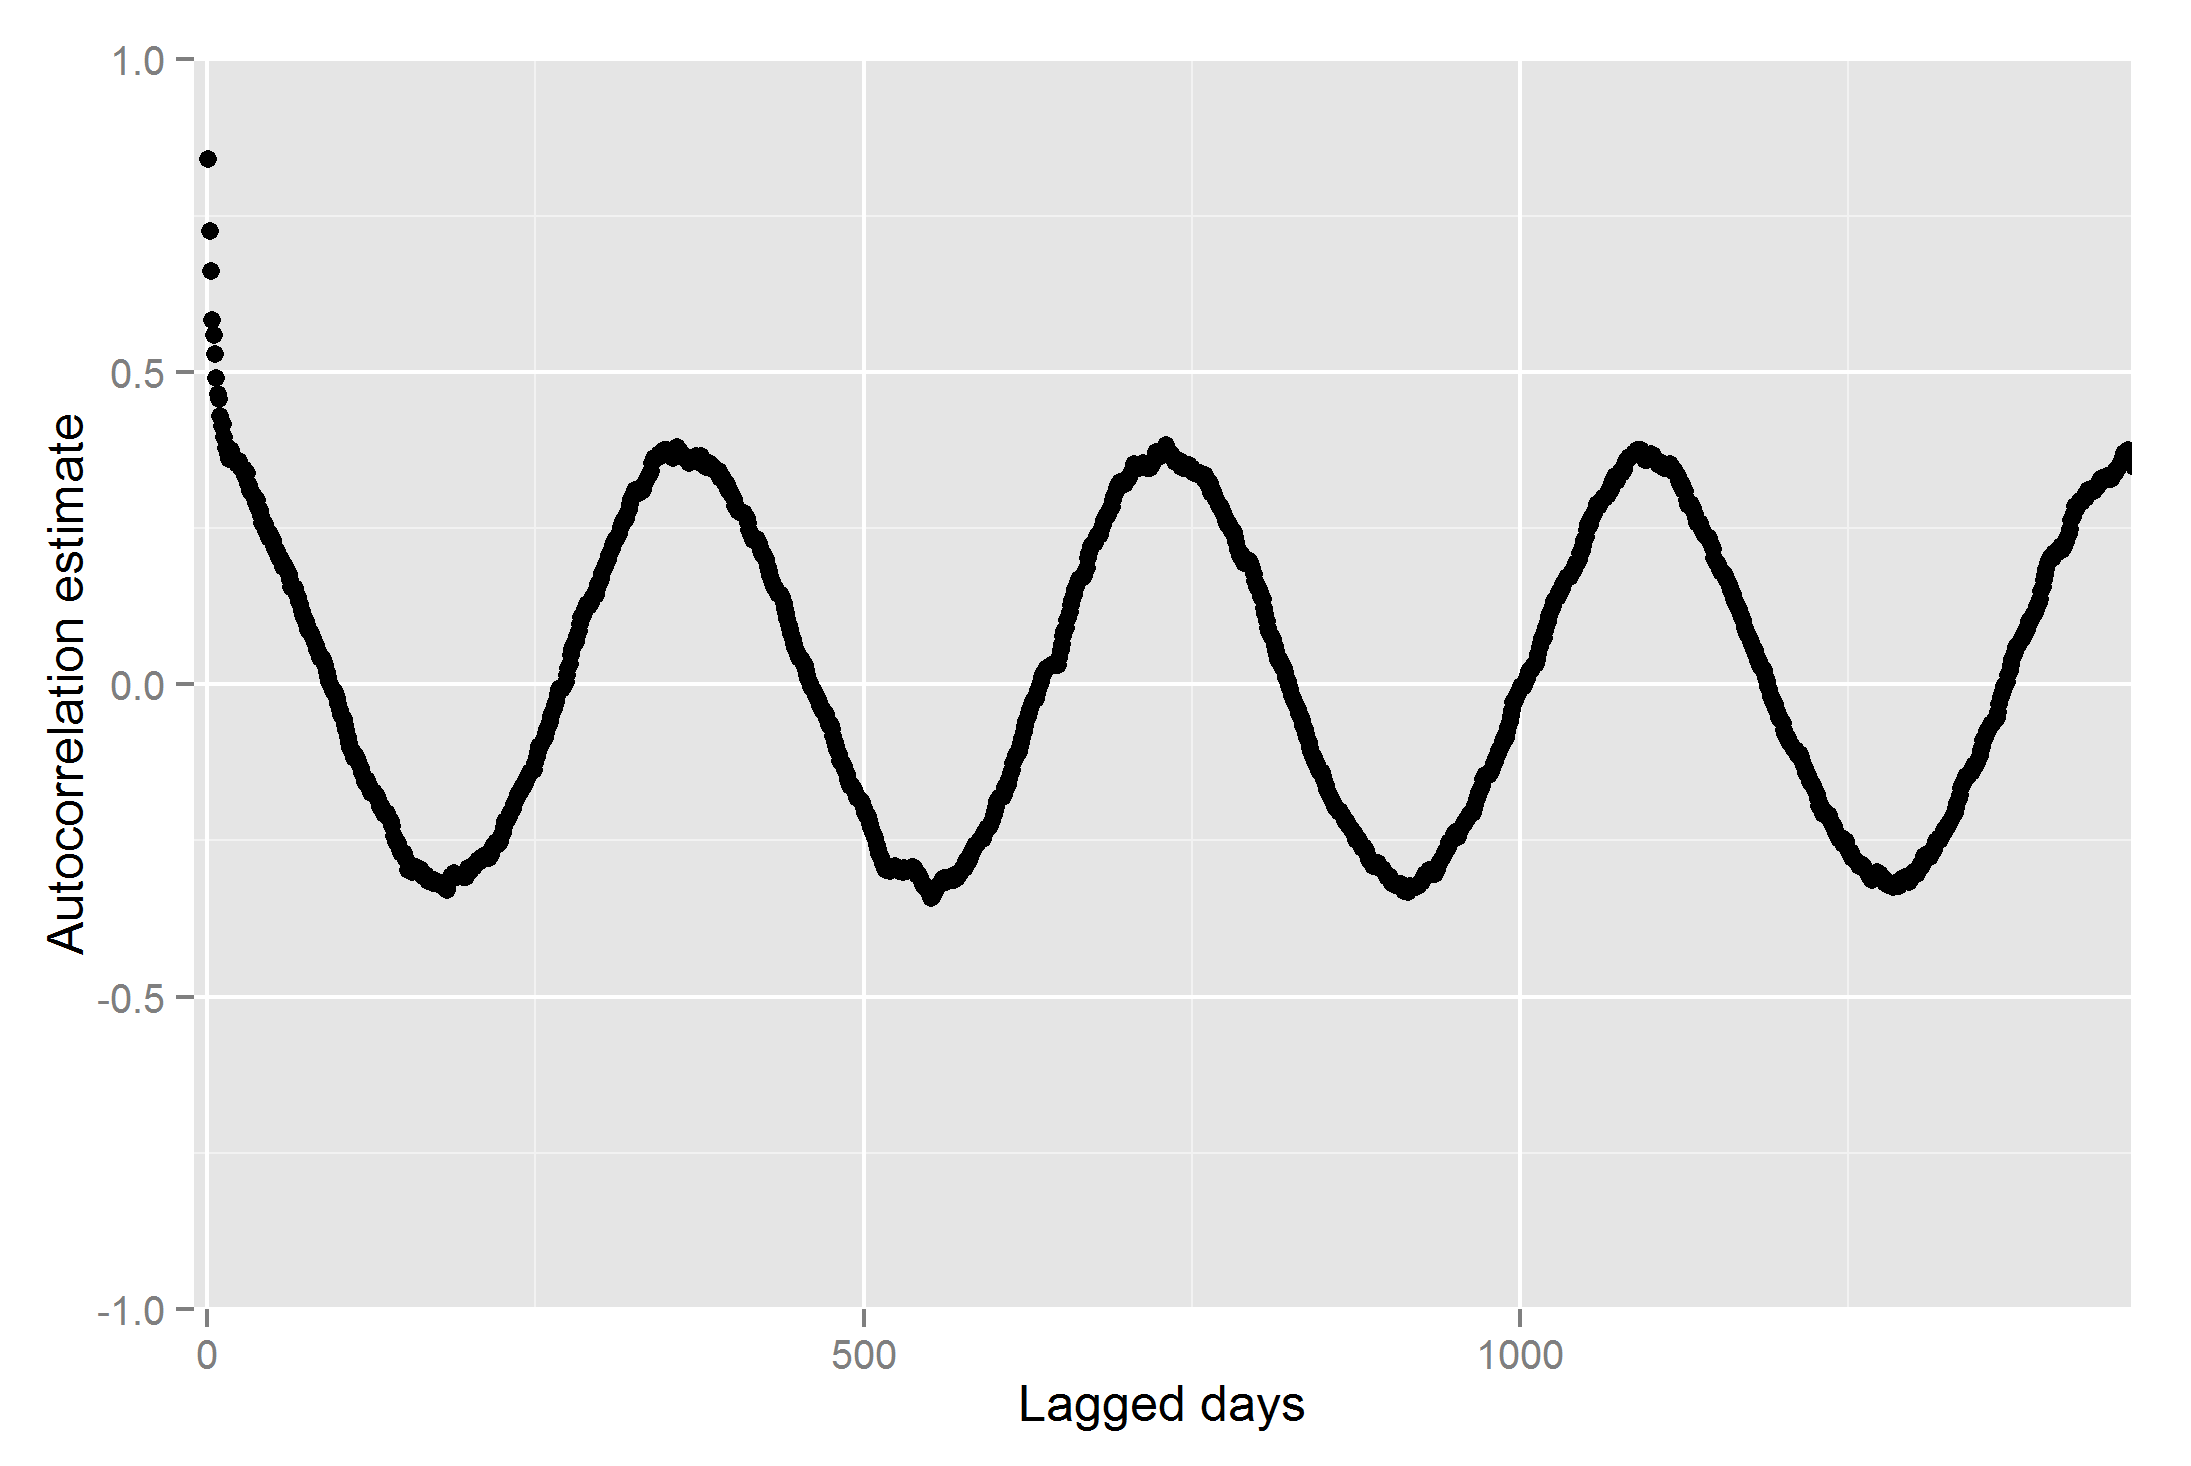
\includegraphics[width=.8\textwidth]{Autocorrelation_function_short_35121_100}
	\end{figure}
	\begin{itemize}
		\item To estimate $\Sigma$ (from the previous slide), I'll model the autocorrelation function individually for each series.
		\item The plot above depicts the autocorrelation estimated at one particular station.
	\end{itemize}
}

\end{document}